\thispagestyle{thachthuctoanhocnone}
\pagestyle{thachthuctoanhoc}
\everymath{\color{thachthuctoanhoc}}
\graphicspath{{../thachthuctoanhoc/pic/}}
\begingroup
\AddToShipoutPicture*{\put(0,616){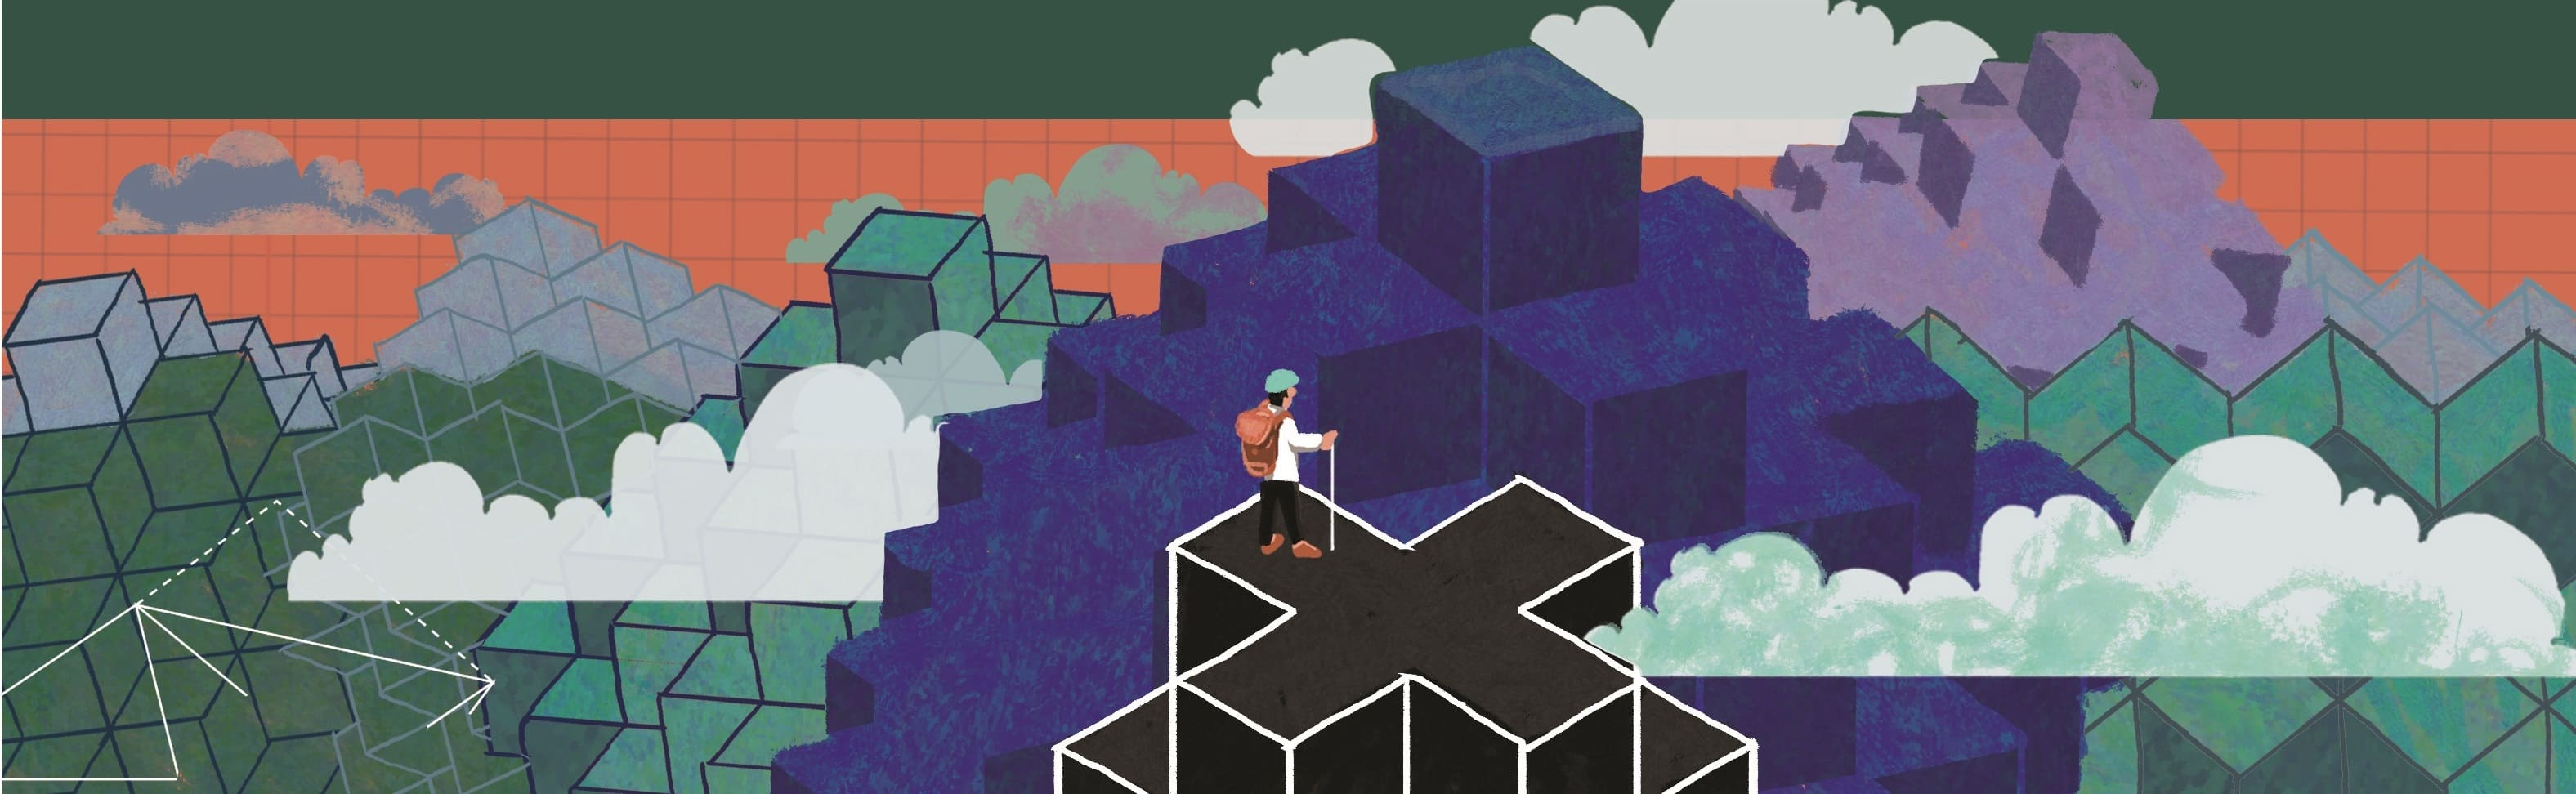
\includegraphics[width=19.3cm]{../thachthuctoanhoc/bannerthachthuc}}}
\centering
\vspace*{4cm}
\endgroup
\vspace*{-8pt}
\begin{tBox}
	\begin{itemize}[leftmargin = 13pt, itemsep = 1.0pt] 
		\item Mỗi bài toán đề xuất (kèm theo lời giải) cần được nêu rõ là bài sáng tác hay bài sưu tầm.
%				\item Mỗi bài toán đề xuất (kèm theo lời giải) cần được nêu rõ là bài sáng tác hay bài sưu tầm (nếu là bài sưu tầm, cần ghi rõ nguồn).
		\item Bài giải cho mỗi bài toán cần được trình bày trong một file riêng hoặc
		một tờ giấy riêng.
		\item  Người đề xuất bài toán hoặc gửi bài giải cho các bài toán trong mục ``Thách thức kỳ này" cần ghi rõ họ, đệm, tên và nơi làm việc/học tập, số điện thoại liên hệ. Nếu là học sinh (hoặc sinh viên) cần ghi rõ là học sinh lớp mấy (hoặc sinh viên năm thứ mấy).
		\item Các bài toán trong mục Thách thức kỳ này hướng tới các độc giả là học sinh phổ thông; được phân chia thành các mức độ $B$, $A$, và được sắp xếp theo độ khó tăng dần, theo đánh giá chủ quan của Ban biên tập. Các bài toán mức độ $B$ không đòi hỏi các kiến thức vượt quá chương trình môn Toán cấp THCS; các bài toán mức độ $A$ không đòi hỏi các kiến thức vượt quá chương trình môn Toán cấp THPT.
		\item Cách thức gửi bài toán đề xuất hoặc lời giải: gửi file thu được bằng cách scan, ảnh chụp (rõ nét) của bản viết tay, hoặc được soạn thảo bằng các phần mềm Latex, Word tới \url{bbt@pi.edu.vn} hoặc gửi qua đường bưu điện tới Tòa soạn (xem địa chỉ tại bìa $2$).
		\item Hạn gửi lời giải cho các bài toán P$681$--P$690$: trước ngày $15/4/2023$.
	\end{itemize}
\end{tBox}
\begin{center}
	\vspace*{-5pt}
	\textbf{\color{thachthuctoanhoc}\color{thachthuctoanhoc}\color{thachthuctoanhoc}THÁCH THỨC KỲ NÀY}
	\vspace*{-5pt}
\end{center}
\begin{multicols}{2}
	\setlength{\abovedisplayskip}{4pt}
	\setlength{\belowdisplayskip}{4pt}
	{\color{thachthuctoanhoc}{\usefont{T5}{qag}{b}{n} P681.}}
	(Mức $B$) Một số có bốn chữ số $\overline{a b c d}$ được gọi là số ``zig zag", nếu $a, b, c, d$ đôi một khác nhau, và $a<b, b>c, c<d$ (chẳng hạn, $1204$ là số ``zig zag"). Hỏi có bao nhiêu số ``zig zag" có chữ số hàng nghìn là $7$?
	\begin{flushright}
		\textit{\small{Trích Đề thi VMTC $2022$--Vòng $1$--Khối lớp $6$}}
	\end{flushright}
	{\color{thachthuctoanhoc}{\usefont{T5}{qag}{b}{n} P682.}}
	(Mức $B$) Cho $100$ số hữu tỷ $a_1,a_2,\ldots,a_{100}$ thoả mãn $a_1+a_4=4$ và
	\begin{align*}
		\dfrac{a_1+a_2}1=\dfrac{a_2+a_3}2=\cdots=\dfrac{a_{100}+a_1}{100}
	\end{align*}
	Tính tổng $a_1+\cdots+a_{100}$. 
	\begin{flushright}
		\textit{\small{Trích Đề thi VMTC $2022$--Vòng $1$--Khối lớp $7$}}
	\end{flushright}
	{\color{thachthuctoanhoc}{\usefont{T5}{qag}{b}{n} P683.}}
	(Mức $B$) Cho tam giác nhọn $ABC$, với $AB<AC$, nội tiếp $(O)$. Gọi $M$ là trung điểm của cạnh $BC$. Trên đoạn thẳng $AM$, lấy điểm $D$ sao cho $\angle CBD=\angle BAM$. Các đường thẳng $BD$, $CD$ lần lượt cắt $(O)$ tương ứng tại các điểm thứ hai $E$, $F$. Chứng minh rằng $AM$ là phân giác của góc $\angle EAF$. 
	\begin{figure}[H]
		\centering
		\vspace*{-5pt}
		\captionsetup{labelformat= empty, justification=centering}
		\definecolor{qqzzff}{rgb}{0,0.6,1}
		\definecolor{ffqqqq}{rgb}{1,0,0}
		\definecolor{qqqqff}{rgb}{0,0,1}
		\definecolor{qqqqffa}{rgb}{1,1,1}
		\begin{tikzpicture}[thachthuctoanhoc,scale=0.7]
			\draw [shift={(-5.18,-1)}] (0,0) -- (0:0.5) arc (0:37.231448415277484:0.5) -- cycle;
			\draw [shift={(-3.82,3.58)}] (0,0) -- (-106.53843051971272:0.5) arc (-106.53843051971272:-69.30698210443525:0.5) -- cycle;
			\draw  (-3.82,3.58)-- (-5.18,-1);
			\draw  (1,-1)-- (-3.82,3.58);
			\draw [color=ffqqqq] (-2.09,0.5743668122270744) circle (3.4679577361095446cm);
			\draw [color=qqzzff] (-3.82,3.58)-- (-2.09,-1);
			\draw  (-5.244701082585602,2.0147111943021647)-- (-3.82,3.58);
			\draw  (-3.82,3.58)-- (0.2545296650521489,3.129735965428329);
			\draw [color=qqzzff] (-5.244701082585602,2.0147111943021647)-- (1,-1);
			\draw [color=qqzzff] (-5.18,-1)-- (0.2545296650521489,3.129735965428329);
			\draw [shift={(-5.18,-1)}] (0:0.5) arc (0:37.231448415277484:0.5);
			\draw (-4.763020430671502,-0.8595434630833395) -- (-4.649298729945548,-0.8212371348333412);
			\draw [shift={(-3.82,3.58)}] (-106.53843051971272:0.5) arc (-106.53843051971272:-69.30698210443525:0.5);
			\draw (-3.8040510242803056,3.1402891516308777) -- (-3.799701303629479,3.020368011166572);
			\draw  (-5.18,-1)-- (-2.09,-1);
			\draw  (-3.675,-0.9) -- (-3.675,-1.1);
			\draw  (-3.595,-0.9) -- (-3.595,-1.1);
			\draw  (-2.09,-1)-- (1,-1);
			\draw  (-0.585,-0.9) -- (-0.585,-1.1);
			\draw  (-0.505,-0.9) -- (-0.505,-1.1);
			\draw [fill=qqqqffa] (-3.82,3.58) circle (1.6pt);
			\draw[color=qqqqff] (-4.02,4.05) node {$A$};
			\draw [fill=qqqqffa] (-5.18,-1) circle (1.6pt);
			\draw[color=qqqqff] (-5.56,-1.17) node {$B$};
			\draw [fill=qqqqffa] (1,-1) circle (1.6pt);
			\draw[color=qqqqff] (1.22,-1.19) node {$C$};
			\draw [fill=qqqqffa] (-2.09,-1) circle (1.6pt);
			\draw[color=qqqqff] (-2.16,-1.29) node {$M$};
			\draw [fill=qqqqffa] (-2.7791404004288816,0.8244294994013176) circle (1.6pt);
			\draw[color=qqqqff] (-2.98,0.45) node {$D$};
			\draw [fill=qqqqffa] (-5.244701082585602,2.0147111943021647) circle (1.6pt);
			\draw[color=qqqqff] (-5.64,2.27) node {$F$};
			\draw [fill=qqqqffa] (0.2545296650521489,3.129735965428329) circle (1.6pt);
			\draw[color=qqqqff] (0.48,3.51) node {$E$};
		\end{tikzpicture}
		\vspace*{-10pt}
	\end{figure}
	\begin{flushright}
		\textit{\small Bằng Linh, Phú Thọ}
	\end{flushright}
	{\color{thachthuctoanhoc}{\usefont{T5}{qag}{b}{n} P684.}}
	(Mức $B$) Tập các điểm trong mặt phẳng toạ độ $Oxy$, có toạ độ thoả mãn phương trình $\left(x^2+y^2-4\right)^3= x^2y^3$ là một đường ``trái tim" như dưới đây. Hãy xác định tất cả các điểm nguyên thuộc đường đó? 
	\vskip 0.05cm
	({\it Điểm nguyên là điểm có cả hoành độ và tung độ đều là các số nguyên}).
	\begin{figure}[H]
		\centering
		\vspace*{-5pt}
		\captionsetup{labelformat= empty, justification=centering}
		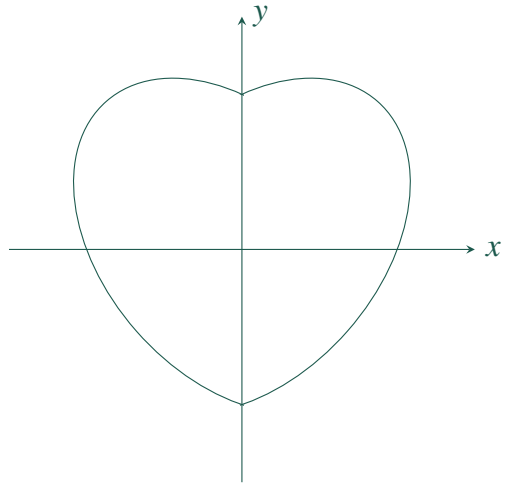
\includegraphics[width=0.8\linewidth]{P1}
	\end{figure}
	\begin{flushright}
		\textit{\small{Trích Đề thi VMTC $2022$--Vòng $1$--Khối lớp $9$}}
	\end{flushright}
	{\color{thachthuctoanhoc}{\usefont{T5}{qag}{b}{n} P685.}}
	(Mức $B$) Trong một hình vuông diện tích $1$ chứa $2023$ hình có tổng diện tích lớn hơn $2022$. Chứng minh rằng, tất cả các hình này có một điểm chung.
	\begin{flushright}
		\textit{\small Duy Minh, Hà Nội (st)}
	\end{flushright}
	{\color{thachthuctoanhoc}{\usefont{T5}{qag}{b}{n} P686.}}
	(Mức $B$) Cho $a,b,c$ là các số thực dương. Chứng minh rằng
	\begin{align*}
		&\dfrac{\sqrt{b c}}{a\!+\!\sqrt{(a\!+\!b)(a\!+\!c)}}+\dfrac{\sqrt{c a}}{b+\sqrt{(b+c)(b+a)}}\\
		&+\dfrac{\sqrt{a b}}{c+\sqrt{(c+a)(c+b)}} \geq 1.
	\end{align*}
	\begin{flushright}
		\textit{\small Nguyễn Việt Hùng, Hà Nội}
	\end{flushright}
	{\color{thachthuctoanhoc}{\usefont{T5}{qag}{b}{n} P687.}}
	(Mức $A$) Tìm tất cả các cặp số thực $(p;q)$, sao cho phương trình $x^3-px+q=0$ có ba nghiệm thực $a,b,c$ ($a<b<c$) thoả mãn:
	\begin{align*}
		a^2-b=b^2-c=c^2-a.
	\end{align*}
	\hfill	\textit{\small{Nguyễn Anh Vũ, Bình Định}}
	\vskip 0.1cm
	\columnbreak
	{\color{thachthuctoanhoc}{\usefont{T5}{qag}{b}{n} P688.}}
	(Mức $A$) Chứng minh rằng, không tồn tại dãy vô hạn các số nguyên tố đôi một phân biệt, mà hai số hạng liên tiếp bất kỳ trong dãy sai khác nhau không quá $2023$. 
	\begin{flushright}
		\textit{Trần Nam Hải, Nam Định}
	\end{flushright}
	{\color{thachthuctoanhoc}{\usefont{T5}{qag}{b}{n} P689.}}
	(Mức $A$) Cho tam giác nhọn $ABC$, với $AB<AC$, nội tiếp $(O)$ và có hai đường cao $BE,CF$ cắt nhau tại $H$.  Đường thẳng $AH$ cắt $(O)$ tại điểm thứ hai $K$. Đường thẳng $KE$ cắt đường tròn ngoại tiếp tam giác $AEF$ tại điểm thứ hai $G$; đường thẳng $CG$ cắt đường tròn ngoại tiếp tam giác $AEF$ tại điểm thứ hai $I$.  Các đường thẳng $AI$ và $BC$ cắt nhau tại $M$. Chứng minh rằng các đường thẳng $BC,MH,BK$ đồng quy. 
	\begin{figure}[H]
		\centering
		\vspace*{-5pt}
		\captionsetup{labelformat= empty, justification=centering}
		\definecolor{qqzzff}{rgb}{0,0.6,1}
		\definecolor{ffqqqq}{rgb}{1,0,0}
		\definecolor{qqqqff}{rgb}{0,0,1}
		\definecolor{qqqqffa}{rgb}{1,1,1}
		\begin{tikzpicture}[thachthuctoanhoc,scale=0.5, node font=\small]
			\draw[] (-2.317157287525381,-1.62) -- (-2.317157287525381,-1.3371572875253814) -- (-2.6,-1.3371572875253814) -- (-2.6,-1.62) -- cycle; 
			\draw[] (0.012081063823149135,1.7891093432485716) -- (0.195227531820648,1.5735696224079776) -- (0.4107672526612419,1.7567160904054766) -- (0.22762078466374303,1.9722558112460704) -- cycle; 
			\draw [,color=ffqqqq] (-0.36,1.2452023121387283) circle (4.632384298553513cm);
			\draw [] (-2.6,5.3)-- (-4,-1.62);
			\draw [] (-4,-1.62)-- (3.28,-1.62);
			\draw [] (3.28,-1.62)-- (-2.6,5.3);
			\draw [,color=qqzzff] (-2.6,-1.62)-- (-2.6,5.3);
			\draw [,color=qqzzff] (0.22762078466374303,1.9722558112460704)-- (-4,-1.62);
			\draw [,color=qqzzff] (-3.7137446234833402,-0.20508056750337042)-- (3.28,-1.62);
			\draw [,color=qqzzff] (-2.6,-2.8095953757225436)-- (-2.6,-1.62);
			\draw [] (-2.6,-2.8095953757225436)-- (0.22762078466374303,1.9722558112460704);
			\draw [] (-2.6,2.4347976878612716) circle (2.865202312138728cm);
			\draw [] (-5.455875353032386,2.203799295167169)-- (3.28,-1.62);
			\draw [] (-8.982873504336062,-1.62)-- (-2.6,5.3);
			\draw [] (-8.982873504336062,-1.62)-- (-4,-1.62);
			\draw [,dashed] (-8.982873504336062,-1.62)-- (-2.6,-0.4304046242774565);
			\draw [,dashed] (-4.89632998688517,-0.8583785660571098)-- (0.22762078466374303,1.9722558112460704);
			\draw [,dash pattern=on 1pt off 3.6pt] (-4.89632998688517,-0.8583785660571098)-- (-2.6,-2.8095953757225436);
			\draw [fill=qqqqffa] (-2.6,5.3) circle (1.6pt);
			\draw[color=qqqqff] (-2.74,5.83) node {$A$};
			\draw [fill=qqqqffa] (-4,-1.62) circle (1.6pt);
			\draw[color=qqqqff] (-4.4,-2.25) node {$B$};
			\draw [fill=qqqqffa] (3.28,-1.62) circle (1.6pt);
			\draw[color=qqqqff] (3.66,-1.87) node {$C$};
			\draw [fill=qqqqffa] (-2.6,-1.62) circle (1.6pt);
			\draw[color=qqqqff] (-3,-1.25) node {$D$};
			\draw [fill=qqqqffa] (0.22762078466374303,1.9722558112460704) circle (1.6pt);
			\draw[color=qqqqff] (0.8,2.27) node {$E$};
			\draw [fill=qqqqffa] (-3.7137446234833402,-0.20508056750337042) circle (1.6pt);
			\draw[color=qqqqff] (-3.86,0.47) node {$F$};
			\draw [fill=qqqqffa] (-2.6,-0.4304046242774565) circle (1.6pt);
			\draw[color=qqqqff] (-2.86,-0.05) node {$H$};
			\draw [fill=qqqqffa] (-2.6,-2.8095953757225436) circle (1.6pt);
			\draw[color=qqqqff] (-3,-3.27) node {$K$};
			\draw [fill=qqqqffa] (-0.832204519089911,0.17996212242440804) circle (1.6pt);
			\draw[color=qqqqff] (-0.78,-0.35) node {$G$};
			\draw [fill=qqqqffa] (-5.455875353032386,2.203799295167169) circle (1.6pt);
			\draw[color=qqqqff] (-5.86,2.37) node {$I$};
			\draw [fill=qqqqffa] (-8.982873504336062,-1.62) circle (1.6pt);
			\draw[color=qqqqff] (-9.4,-2.25) node {$M$};
			\draw [fill=qqqqffa] (-4.89632998688517,-0.8583785660571098) circle (1.6pt);
		\end{tikzpicture}
		\vspace*{-10pt}
	\end{figure}
	\begin{flushright}
		\textit{\small Nguyễn Khang, Cần Thơ}
	\end{flushright}
	{\color{thachthuctoanhoc}{\usefont{T5}{qag}{b}{n} P690.}}
	(Mức $A$) Có $20$ tấm bìa, được đánh số thứ tự từ $1$ đến $20$. Với mỗi $m=1,2,\ldots,20$, người ta viết lên tấm bìa thứ $m$ một số thực có phần nguyên bằng $m$. Chứng minh rằng, có thể chọn ra bốn tấm bìa, mà tổng hai số được viết ở hai trong bốn tấm ấy và tổng hai số được viết ở hai tấm còn lại sai khác nhau dưới $\dfrac16$.
	\begin{flushright}
		\textit{\small{Trần Nam Dũng, Tp. Hồ Chí Minh (st)}}
	\end{flushright}
\end{multicols}
\newpage
\centerline{{\large{\textbf{\color{thachthuctoanhoc}GIẢI BÀI KỲ TRƯỚC}}}}
\vspace*{-5pt}
\begin{multicols}{2}
	\setlength{\abovedisplayskip}{4pt}
	\setlength{\belowdisplayskip}{4pt}
	{\color{thachthuctoanhoc}{\usefont{T5}{qag}{b}{n} P651.}}
	(Mức $B$)
	Có hai chiếc hộp, mỗi hộp đều chứa các viên bi khác màu. Số viên bi đỏ ở hộp thứ nhất bằng $\dfrac{4}{15}$ số viên bi trong hộp đó. Tổng số viên bi đỏ ở hai hộp bằng $\dfrac{11}{25}$ tổng số viên bi của hai hộp. Hỏi, trong hai hộp có ít nhất bao nhiêu viên bi đỏ? Biết rằng, hộp thứ hai chứa $200$ viên bi.
	\vskip 0.05cm
	\textbf{\color{thachthuctoanhoc}Lời giải} (\textit{của người chấm bài})\textbf{\color{thachthuctoanhoc}.}
	\vskip 0.05cm
	Gọi $a$ (viên) là số viên bi đỏ có trong hộp thứ nhất, và gọi $s$ (viên) là tổng số viên bi đỏ của cả hai hộp; ta có, $a, s \in \mathbb{N^*}$. Theo bài ra, ta cần tìm giá trị nhỏ nhất của $s$.
	\vskip 0.05cm
	Vì số viên bi đỏ ở hộp thứ nhất bằng $\dfrac{4}{15}$  số viên bi trong hộp đó, nên số viên bi có trong hộp thứ nhất bằng  $\dfrac{15a}{4}$. Do đó, theo giả thiết về tổng số viên bi đỏ của cả hai hộp, ta có:
	\begin{align*}
		s = \dfrac{{11}}{{25}}\left( {\dfrac{{15a}}{4} + 200} \right) = \dfrac{{33a}}{{20}} + 88. \tag{$1$}
	\end{align*}
	Từ đó, do $s \in \mathbb{N^*}$ và $a > 0$, suy ra  $\dfrac{33a}{20} \in \mathbb{N^*}$. Vì thế, $33a$ chia hết cho $20$; mà $(33, 20) = 1$, nên $a$ chia hết cho $20$. Suy ra, $a \ge 20$ (do  $a \in \mathbb{N^*}$). Vì vậy, từ ($1$) ta có:
	\begin{align*}
		s \ge \dfrac{{33 \cdot 20}}{{20}} + 88 = 121. \tag{$2$}	
	\end{align*}
	Tiếp theo, xét hai hộp bi, mà hộp thứ nhất chứa $75$ viên, trong đó có $20$ viên bi đỏ, và hộp thứ hai chứa $200$ viên, trong đó có $101$ viên bi đỏ, ta có:
	\begin{align*}
		20 = \dfrac{4}{{15}} \cdot 75 \text{ và } 20 + 101 = \dfrac{{11}}{{25}}\left( {75 + 200} \right).
	\end{align*}
	Như vậy, hai hộp bi nói trên thỏa mãn tất cả các giả thiết của đề bài, và có tổng số viên bi đỏ ở cả hai hộp bằng $121$ viên. \hfill ($3$)
	\vskip 0.05cm
	Từ ($2$) và ($3$) suy ra, giá trị nhỏ nhất của $s$ là $121$. Nói một cách khác, trong hai hộp bi, thỏa mãn các giả thiết của đề bài, có ít nhất $121$ viên bi đỏ.
	\vskip 0.05cm
	\columnbreak
	\textbf{\color{thachthuctoanhoc}Bình luận và Nhận xét}
	\vskip 0.05cm	
	Rất tiếc, tất cả các lời giải Tạp chí đã nhận được từ bạn đọc đều không được coi là lời giải đúng, do người giải bài đã mắc một trong các lỗi sau:
	\vskip 0.05cm
	-- Khẳng định giá trị nhỏ nhất của $s$ (theo ký hiệu trong Lời giải trên) là $121$ \textit{ngay sau khi} chỉ mới chứng minh được $s \ge 121$;
	\vskip 0.05cm
	(\textit{Lỗi trên đây đã được nhắc nhở nhiều lần trong các số trước đây của Tạp chí!})
	\vskip 0.05cm
	-- Giải một bài toán khác, thay vì giải bài đã ra. Cụ thể, các bạn mắc lỗi này đã giải một trong hai bài toán dưới đây:
	\vskip 0.05cm
	+ Bài toán $1$: Với hai hộp bi thỏa mãn các giả thiết của bài đã ra, hãy tìm số viên bi đỏ nhỏ nhất có thể trong mỗi hộp.
	\vskip 0.05cm
	+ Bài toán $2$: Là bài toán nhận được từ bài đã ra, bằng cách thay giả thiết ``tổng số viên bi đỏ ở hai hộp bằng $\dfrac{11}{25}$ tổng số viên bi của hai hộp" bởi giả thiết ``số viên bi đỏ ở hộp thứ hai bằng $\dfrac{11}{25}$  tổng số viên bi của hai hộp".
	\vskip 0.1cm
		\hfill\textbf{\color{thachthuctoanhoc}Lê Huy}
	\vskip 0.1cm
	{\color{thachthuctoanhoc}{\usefont{T5}{qag}{b}{n} P652.}}
	(Mức $B$) Chứng minh rằng, với hai số nguyên dương $a$, $b$, ta có thể tìm được số nguyên dương $c$, sao cho $a^2 + b^2 + c^2$  là một số chính phương, khi và chỉ khi $ab$ là một số chẵn.
	\vskip 0.05cm
	\textbf{\color{thachthuctoanhoc}Lời giải} (\textit{dựa theo các lời giải đúng, mà Tạp chí đã nhận được từ bạn đọc})\textbf{\color{thachthuctoanhoc}.}
	\vskip 0.05cm
	$\pmb{1.}$ \textit{Chứng minh ``khi".
	\vskip 0.05cm
	Giả sử $a$, $b$ là hai số nguyên dương có tích là một số chẵn. Ta cần chứng minh có thể tìm được số nguyên dương $c$, sao cho $a^2 + b^2 + c^2$  là một số chính phương.}
	\vskip 0.05cm
	Vì $ab$ là một số chẵn nên trong hai số nguyên dương $a$, $b$ có ít nhất một số chẵn. Do đó, xảy ra một trong hai trường hợp sau:
	\vskip 0.05cm
	$\diamond$ \textit{Trường hợp} $1$: Trong hai số $a$, $b$ có đúng một số chẵn.
	\vskip 0.05cm
	Khi đó, $a^2 + b^2$ là một số nguyên dương lẻ. Vì thế, tồn tại số nguyên dương $m$, sao cho
	\begin{align*}
		{a^2} + {b^2} = 2m + 1.
	\end{align*}
	Chọn $c = m$, ta có $c$ là số nguyên dương, và
	\begin{align*}
		{a^2} + {b^2} + {c^2} = 2m + 1 + {m^2} = {\left( {m + 1} \right)^2},
	\end{align*}
	là một số chính phương.
	\vskip 0.05cm
	$\diamond$ \textit{Trường hợp} $2$: Cả hai số $a$, $b$ đều là số chẵn.
	\vskip 0.05cm
	Khi đó, $a^2, b^2$  là các số chẵn chia hết cho $4$. Suy ra, $a^2 + b^2$ là một số nguyên dương chẵn chia hết cho $4$, và lớn hơn hoặc bằng $8$. Vì thế, tồn tại số nguyên dương $k \ge 2$, sao cho
	\begin{align*}
		{a^2} + {b^2} = 4k.
	\end{align*}
	Chọn $c = k - 1$, ta có $c$ là số nguyên dương, và
	\begin{align*}
		{a^2} + {b^2} + {c^2} = 4k + {\left( {k - 1} \right)^2} = {\left( {k + 1} \right)^2},
	\end{align*}
	là một số chính phương.
	\vskip 0.05cm
	Hiển nhiên, kết quả xét hai trường hợp trên cho ta điều cần chứng minh.
	\vskip 0.05cm
	$\pmb{2.}$ \textit{Chứng minh ``chỉ khi".}
	\vskip 0.05cm
	\textit{Giả sử $a$, $b$ là hai số nguyên dương, sao cho có số nguyên dương $c$, để $a^2 + b^2 + c^2$  là một số chính phương. Ta cần chứng minh ab là một số chẵn.}
	\vskip 0.05cm
	Giả sử $ab$ là một số lẻ. \hfill ($1$)
	\vskip 0.05cm
	Khi đó, cả hai số $a$, $b$ đều là số lẻ. Do đó, số dư trong các phép chia  $a^2$, $b^2$ cho $4$ đều là $1$. Suy ra, số dư trong phép chia $a^2 + b^2$  cho $4$ là $2$. Từ đây, do số dư trong phép chia $c^2$ cho $4$ là $0$ hoặc $1$, nên số dư trong phép chia $a^2 + b^2 + c^2$  cho $4$ sẽ là $2$ hoặc $3$. \hfill ($2$)
	\vskip 0.05cm
	Mặt khác, do $a^2 + b^2 + c^2$ là một số chính phương, nên số dư trong phép chia  $a^2 + b^2 + c^2$ cho $4$ chỉ có thể là $0$ hoặc $1$, mâu thuẫn \linebreak với ($2$).
	\vskip 0.05cm
	Mâu thuẫn nhận được chứng tỏ giả sử ($1$) là sai. Vì thế, ta có điều cần chứng minh.
	\vskip 0.05cm
	\textbf{\color{thachthuctoanhoc}Bình luận và Nhận xét}
	\vskip 0.05cm
	Rất tiếc, có hơn nửa số lời giải, trong số tất cả các lời giải Tạp chí đã nhận được từ bạn đọc, là lời giải không đúng, do người giải bài đã mắc một trong các lỗi sau:
	\vskip 0.05cm
	-- Ở phần chứng minh ``khi", chưa chứng minh số $c$ được chọn là số dương;
	\vskip 0.05cm
	-- Chỉ mới chứng minh hoặc ``khi", hoặc ``chỉ khi".
	\vskip 0.1cm
		\hfill\textbf{\color{thachthuctoanhoc}Lưu Thị Thanh Hà}
	\vskip 0.1cm
	{\color{thachthuctoanhoc}{\usefont{T5}{qag}{b}{n} P653.}}
	(Mức $B$)
	Cho hình chữ nhật $ABCD$. Gọi $E$ là hình chiếu vuông góc của điểm $B$ trên đường thẳng $AC$; $F$ là trung điểm của đoạn $AE$. Các đường thẳng $BF$, $AD$ cắt nhau tại $G$. Gọi $K$ là trung điểm của $AG$. Chứng minh rằng, $DK + KF > CF$.
	\vskip 0.05cm
	\textbf{\color{thachthuctoanhoc}Lời giải} (\textit{dựa theo lời giải của bạn Nguyễn Minh Tuấn, lớp $9$B, trường THPT chuyên Hà Nội -- Amsterdam, Tp. Hà Nội})\textbf{\color{thachthuctoanhoc}.}
	\begin{figure}[H]
		\vspace*{-10pt}
		\centering
		\captionsetup{labelformat= empty, justification=centering}
		\definecolor{ffqqqq}{rgb}{1.,0.,0.}
		\definecolor{qqwuqq}{rgb}{0.,0.39215686274509803,0.}
		\definecolor{uuuuuu}{rgb}{0.26666666666666666,0.26666666666666666,0.26666666666666666}
		\definecolor{xdxdff}{rgb}{0.49019607843137253,0.49019607843137253,1.}
		\definecolor{qqqqff}{rgb}{0.,0.,1.}
		\begin{tikzpicture}[scale=0.65,thachthuctoanhoc, node font=\small]
			\draw[,pattern color=qqwuqq,fill=qqwuqq,fill opacity=0.10000000149011612] (2.389185516011975,2.0738763226586836) -- (2.546078424122522,2.3092156848245047) -- (2.310739061956701,2.466108592935052) -- (2.1538461538461537,2.230769230769231) -- cycle; 
			\draw[,pattern color=qqwuqq,fill=qqwuqq,fill opacity=0.10000000149011612] (2.153846153846154,5.28284271247462) -- (1.8710034413715348,5.28284271247462) -- (1.871003441371535,5.) -- (2.153846153846154,5.) -- cycle; 
			\draw[,pattern color=qqwuqq,fill=qqwuqq,fill opacity=0.10000000149011612] (2.1538461538461537,3.8982273278592343) -- (1.8710034413715346,3.8982273278592348) -- (1.8710034413715346,3.6153846153846154) -- (2.1538461538461537,3.6153846153846154) -- cycle; 
			\draw[,pattern color=qqwuqq,fill=qqwuqq,fill opacity=0.10000000149011612] (4.,3.8982273278592343) -- (3.7171572875253807,3.8982273278592348) -- (3.7171572875253807,3.6153846153846154) -- (4.,3.6153846153846154) -- cycle; 
			\draw[,pattern color=qqwuqq,fill=qqwuqq,fill opacity=0.10000000149011612] (2.650479639749056,4.823641020711007) -- (2.383761695961126,4.729505275844679) -- (2.477897440827454,4.462787332056749) -- (2.7446153846153845,4.556923076923077) -- cycle; 
			\draw[,pattern color=ffqqqq,fill=ffqqqq,fill opacity=0.10000000149011612] (2.9827873320567484,3.8821025591725458) -- (2.716069388268818,3.7879668143062175) -- (2.8102051331351463,3.521248870518287) -- (3.0769230769230766,3.6153846153846154) -- cycle; 
			\draw [] (-2.,5.)-- (4.,5.);
			\draw (-2.74,5.86) node[anchor=north west] {$A$};
			\draw (4.,5.72) node[anchor=north west] {$B$};
			\draw (4.,1.24) node[anchor=north west] {$C$};
			\draw (-2.78,1.24) node[anchor=north west] {$D$};
			\draw (1.8,2.16) node[anchor=north west] {$E$};
			\draw (-0.18,4.64) node[anchor=north west] {$F$};
			\draw (-2.78,3.24) node[anchor=north west] {$G$};
			\draw (-2.76,4.38) node[anchor=north west] {$K$};
			\draw [] (2.1538461538461537,2.230769230769231)-- (4.,5.);
			\draw [] (4.,5.)-- (-2.,2.88235294117647);
			\draw [] (-2.,3.941176470588235)-- (-2.,5.);
			\draw [] (-2.09,4.435588235294118) -- (-1.91,4.435588235294118);
			\draw [] (-2.09,4.505588235294118) -- (-1.91,4.505588235294118);
			\draw [] (-2.,3.941176470588235)-- (-2.,2.88235294117647);
			\draw [] (-1.91,3.4467647058823525) -- (-2.09,3.4467647058823525);
			\draw [] (-1.91,3.3767647058823527) -- (-2.09,3.3767647058823527);
			\draw [] (-2.,2.88235294117647)-- (-2.,1.);
			\draw [] (-2.,1.)-- (4.,1.);
			\draw [] (4.,1.)-- (4.,5.);
			\draw [] (0.07692307692307687,3.6153846153846154)-- (2.1538461538461537,2.230769230769231);
			\draw [] (1.107064112441237,3.0367904633030953) -- (1.0072180771206953,2.887021410322283);
			\draw [] (1.1653076330448862,2.9979614495673292) -- (1.0654615977243445,2.848192396586517);
			\draw [] (1.2235511536485353,2.959132435831563) -- (1.1237051183279936,2.809363382850751);
			\draw [] (2.1538461538461537,2.230769230769231)-- (4.,1.);
			\draw [] (0.07692307692307687,3.6153846153846154)-- (-2.,5.);
			\draw [] (-0.9532179585950832,4.193978767466136) -- (-0.853371923274542,4.343747820446948);
			\draw [] (-1.0114614791987322,4.2328077812019025) -- (-0.9116154438781912,4.382576834182714);
			\draw [] (-1.0697049998023813,4.271636794937669) -- (-0.9698589644818402,4.42140584791848);
			\draw [] (-2.,3.941176470588235)-- (0.07692307692307687,3.6153846153846154);
			\draw [] (2.1538461538461537,6.230769230769231)-- (4.,5.);
			\draw [] (2.1538461538461537,6.230769230769231)-- (2.1538461538461537,3.289592760180996);
			\draw [] (2.1538461538461537,3.289592760180996)-- (2.1538461538461537,2.230769230769231);
			\draw [] (4.,1.)-- (2.1538461538461537,6.230769230769231);
			\draw [] (0.07692307692307687,3.6153846153846154)-- (2.1538461538461537,3.289592760180996);
			\draw [] (-2.,1.)-- (2.1538461538461537,6.230769230769231);
			\draw [] (4.,3.6153846153846154)-- (0.07692307692307687,3.6153846153846154);
			\draw (1.54,3.44) node[anchor=north west] {$I$};
			\draw (1.94,6.98) node[anchor=north west] {$J$};
			\draw (3.18,3.68) node[anchor=north west] {$H$};
			\draw (1.52,5.) node[anchor=north west] {$L$};
			\draw [] (3.0769230769230766,3.6153846153846154)-- (2.1538461538461537,3.289592760180996);
			\draw [] (2.1538461538461537,3.289592760180996)-- (4.,1.);
			\draw [fill=qqqqff] (-2.,5.) circle (1.5pt);
			\draw [fill=qqqqff] (4.,5.) circle (1.5pt);
			\draw [fill=xdxdff] (-2.,1.) circle (1.5pt);
			\draw [fill=uuuuuu] (4.,1.) circle (1.5pt);
			\draw [fill=uuuuuu] (2.1538461538461537,2.230769230769231) circle (1.5pt);
			\draw [fill=uuuuuu] (0.07692307692307687,3.6153846153846154) circle (1.5pt);
			\draw [fill=uuuuuu] (-2.,2.88235294117647) circle (1.5pt);
			\draw [fill=uuuuuu] (-2.,3.941176470588235) circle (1.5pt);
			\draw [fill=uuuuuu] (2.1538461538461537,3.289592760180996) circle (1.5pt);
			\draw [fill=xdxdff] (2.1538461538461537,6.230769230769231) circle (1.5pt);
			\draw [fill=uuuuuu] (3.0769230769230766,3.6153846153846154) circle (1.5pt);
			\draw [fill=uuuuuu] (2.153846153846154,4.348416289592761) circle (1.5pt);
		\end{tikzpicture}
		\vspace*{-10pt}
	\end{figure}
	Gọi $I$, $J$ tương ứng là điểm đối xứng với $K$, $D$ qua $F$; ta có:
	\vskip 0.05cm
	+ Đường thẳng $JI$ đối xứng với đường thẳng $DK$ qua $F$; \hfill ($1$)
	\vskip 0.05cm
	+ $JI = DK$. \hfill ($2$)
	\vskip 0.05cm
	Do ($1$) nên gọi $L$ là giao điểm của các đường thẳng $JI$ và $GF$, ta có $L$ đối xứng với $G$ qua $F$. Mà $E$ đối xứng với $A$ qua $F$ (do giả thiết $F$ là trung điểm của $AE$) nên đoạn thẳng $EL$ đối xứng với đoạn thẳng $AG$ qua $F$. Do đó, từ $K$ là trung điểm của $AG$ (giả thiết) suy ra $I$ là trung điểm của $EL$. \hfill ($3$)
	\vskip 0.05cm
	Do $D$, $A$ tương ứng đối xứng với $J$, $E$ qua $F$, nên $AD \parallel JE$ và $AD = JE$. Mà $BC \parallel AD$ và $BC = AD$ (do $ABCD$ là hình chữ nhật), nên $BC \parallel JE$ và $BC = JE$. Do đó, $JBCE$ là hình bình hành. Vì thế, gọi $H$ là giao điểm của $BE$ và $JC$, ta có $H$ là trung điểm của $BE$ và của $CJ$. Suy ra, $IH$ là đường trung bình của tam giác $LEB$ (do ($3$)), và $FH$ là đường trung bình của tam giác $AEB$. Do đó
	\begin{align*}
		IH \parallel FB, \tag{$4$}
	\end{align*}
	và \hspace*{60.5pt}  $FH \parallel AB$. \hfill ($5$)
	\vskip 0.05cm
	Từ ($5$), do $AB \bot BC$, suy ra $FH \bot BC$. Mà $BH \bot FC$ (do giả thiết $E$ là hình chiếu vuông góc của $B$ trên $AC$) nên $H$ là trực tâm của tam giác $BFC$. Do đó, $CH \bot FB$, hay $CJ \bot FB$. \hfill ($6$)
	\vskip 0.05cm
	Từ ($4$) và ($6$), suy ra $IH \bot CJ$. Mà $H$ là trung điểm của $CJ$ (theo chứng minh trên) nên $JIC$ là tam giác cân tại $I$. Vì thế, $IJ = IC$. Kết hợp với ($2$), suy ra $DK = IC$. Do vậy, với lưu ý $KF = IF$, ta có:
	\begin{align*}
		DK + KF = IC + IF > CF.
	\end{align*}
	Ta có điều phải chứng minh theo yêu cầu đề bài.
	\vskip 0.05cm
	\textbf{\color{thachthuctoanhoc}Bình luận và Nhận xét}
	\vskip 0.05cm
	Lời giải của bạn \textit{Nguyễn Minh Tuấn} là lời giải duy nhất Tạp chí nhận được từ bạn đọc.
	\vskip 0.1cm
	\hfill	\textbf{\color{thachthuctoanhoc}Hạ Vũ Anh}
	\vskip 0.1cm
	{\color{thachthuctoanhoc}{\usefont{T5}{qag}{b}{n} P654.}}
	(Mức $B$) Cho đa thức
	\begin{align*}
		f\left( x \right) = 2{x^3} - 3{x^2} + 4x - 5.
	\end{align*}
	Tính tổng
	\begin{align*}
		S =& f\left( {\dfrac{1}{{2023}}} \right) + f\left( {\dfrac{2}{{2023}}} \right) + f\left( {\dfrac{3}{{2023}}} \right) \\
		&+  \cdots  + f\left( {\dfrac{{2022}}{{2023}}} \right).
	\end{align*}
	\textbf{\color{thachthuctoanhoc}Lời giải.}
	\vskip 0.05cm
	$\bullet$ \textbf{\color{thachthuctoanhoc}Cách} $\pmb{1}$ (\textit{dựa theo nhiều lời giải Tạp chí đã nhận được từ bạn đọc})\textbf{\color{thachthuctoanhoc}.}
	\vskip 0.05cm
	Trước hết, ta nhắc lại (không chứng minh) các công thức quen thuộc tính tổng bậc nhất, bậc hai và bậc ba của $n$ số nguyên dương đầu tiên.
	\vskip 0.05cm
	Với $n$ là số nguyên dương tùy ý, ta có:
	\begin{align*}
		&1 + 2 +  \cdots  + n = \dfrac{{n\left( {n + 1} \right)}}{2}\\
		&{1^2} + {2^2} +  \cdots  + {n^2} = \dfrac{{n\left( {n + 1} \right)\left( {2n + 1} \right)}}{6};\\
		&{1^3} + {2^3} +  \cdots  + {n^3} = \dfrac{{{n^2}{{\left( {n + 1} \right)}^2}}}{4}.
	\end{align*}
	Tiếp theo, dễ thấy, ta có:
	\begin{align*}
			S =\, &f\left( {\dfrac{1}{{2023}}} \right) + f\left( {\dfrac{2}{{2023}}} \right) + f\left( {\dfrac{3}{{2023}}} \right) \\
			&+  \cdots  + f\left( {\dfrac{{2022}}{{2023}}} \right)\\
			 =\,\, &2 \cdot \dfrac{1}{{{{2023}^3}}} \cdot \left( {{1^3} + {2^3} + {3^3} +  \cdots  + {{2022}^3}} \right) \\
			 &-\! 3 \!\cdot\! \dfrac{1}{{{{2023}^2}}} \!\cdot\! \left( {{1^2} \!+ {2^2} \!+ {3^2} \!+  \cdots  \!+ {{2022}^2}} \right)\\
			 &+ 4 \cdot \dfrac{1}{{2023}} \cdot \left( {1 + 2 + 3 +  \cdots  + 2022} \right) \\
			 &- 5 \cdot 2022.
	\end{align*}
	Do đó, áp dụng các công thức nêu trên cho $n = 2022$, ta được:
	\begin{align*}
			S =\, &2 \cdot \dfrac{1}{{{{2023}^3}}} \cdot \dfrac{{{{2022}^2} \cdot {{2023}^2}}}{4} \\
			&- 3 \cdot \dfrac{1}{{{{2023}^2}}} \cdot \dfrac{{2022 \cdot 2023 \cdot \left( {2 \cdot 2022 + 1} \right)}}{6} \\
			&+ 4 \cdot \dfrac{1}{{2023}} \cdot \dfrac{{2022 \cdot 2023}}{2} - 5 \cdot 2022\\
			 = \,&\dfrac{{1011 \cdot 2022}}{{2023}} - \dfrac{{1011 \cdot 4045}}{{2023}} \\
			 &+ 2 \cdot 2022 - 5 \cdot 2022\\
			 =  \,&- 1011 + 4 \cdot 1011 - 10 \cdot 1011 =  - 7077.
	\end{align*}
	$\bullet$ \textbf{\color{thachthuctoanhoc}Cách} $2$ (\textit{dựa theo nhiều lời giải Tạp chí đã nhận được từ bạn đọc})\textbf{\color{thachthuctoanhoc}.}
	\vskip 0.05cm
	Trước hết, nhận thấy
	\begin{align*}
		\dfrac{1}{{2023}} + \dfrac{{2022}}{{2023}} &= \dfrac{2}{{2023}} + \dfrac{{2021}}{{2023}} \\
		&=  \cdots  = \dfrac{{1011}}{{2023}} + \dfrac{{1012}}{{2023}} = 1.
	\end{align*}
	Tiếp theo, với $a$, $b$ là hai số thực tùy ý có tổng bằng $1$, ta có:
	\begin{align*}
			&f\left( a \right) + f\left( b \right)\\[-0.3ex]
			 = \,&2\left( {{a^3} \!+\! {b^3}} \right) \!-\! 3\left( {{a^2} \!+\! {b^2}} \right) \!+\! 4\left( {a \!+\! b} \right) \!-\! 10\\[-0.3ex]
			 = \,&2\left( {{{\left( {a + b} \right)}^3} - 3ab\left( {a + b} \right)} \right) \\[-0.3ex]
			 &- 3\left( {{{\left( {a + b} \right)}^2} - 2ab} \right) + 4\left( {a + b} \right) - 10\\[-0.3ex]
			 = \,&2\left( {1 - 3ab} \right) - 3\left( {1 - 2ab} \right) + 4 - 10\\
			 &(\text{{ do }}a + b = 1)\\[-0.3ex]
			 =  \,&- 7.
	\end{align*}
	Do đó
	\begin{align*}
		&f\left( {\dfrac{1}{{2023}}} \right) + f\left( {\dfrac{{2022}}{{2023}}} \right) \\
		= \,&f\left( {\dfrac{2}{{2023}}} \right) + f\left( {\dfrac{{2021}}{{2023}}} \right) \\
		= \,& \cdots  = f\left( {\dfrac{{1011}}{{2023}}} \right) + f\left( {\dfrac{{1012}}{{2023}}} \right) =  - 7.
	\end{align*}
	Vì vậy
	\begin{align*}
			S =\,& \left( {f\left( {\dfrac{1}{{2023}}} \right) + f\left( {\dfrac{{2022}}{{2023}}} \right)} \right) \\
			&+ \left( {f\left( {\dfrac{2}{{2023}}} \right) + f\left( {\dfrac{{2021}}{{2023}}} \right)} \right) \\
			&+  \cdots  + \left( {f\left( {\dfrac{{1011}}{{2023}}} \right) + f\left( {\dfrac{{1012}}{{2023}}} \right)} \right)\\
			 = \,&\left( { - 7} \right) \cdot 1011 =  - 7077.
	\end{align*}
	\textbf{\color{thachthuctoanhoc}Bình luận và Nhận xét}
	\vskip 0.05cm
	$\pmb{1.}$ Với các bạn đọc chưa biết các công thức tính tổng đã nêu ở Cách $1$, các bạn có thể dễ dàng chứng minh các công thức đó bằng phương pháp quy nạp theo $n$.
	\vskip 0.05cm
	$\pmb{2.}$ Cách $1$ là một cách giải rất tự nhiên, và các tính toán trên các số hoàn toàn đơn giản.
	\vskip 0.05cm
	$\pmb{3.}$ Tạp chí đã nhận được rất nhiều lời giải, từ bạn đọc; tất cả các lời giải này đều là lời giải đúng và hoàn chỉnh.
	\vskip 0.1cm
		\hfill\textbf{\color{thachthuctoanhoc}Lê Huy}
	\vskip 0.1cm
	{\color{thachthuctoanhoc}{\usefont{T5}{qag}{b}{n} P655.}}
	(Mức $B$) Tại mỗi đỉnh của một đa giác đều $2023$ cạnh, người ta ghi một số thực, sao cho các số được ghi đôi một khác nhau. Chứng minh rằng, có thể tìm được một tam giác $ABC$ cân tại $A$, với $A$, $B$, $C$ là các đỉnh của đa giác đều đã cho, sao cho số được ghi tại đỉnh $A$ nằm giữa hai số được ghi tại đỉnh $B$ và đỉnh $C$.
	\vskip 0.05cm
	\textbf{\color{thachthuctoanhoc}Lời giải} (\textit{dựa theo lời giải của bạn Phùng Việt Cường, lớp $11$ Toán $2$, trường THPT chuyên Lê Hồng Phong, tỉnh Nam Định})\textbf{\color{thachthuctoanhoc}.}
	\vskip 0.05cm
	Do các số được ghi đôi một khác nhau nên trong các số đó, có đúng một số lớn nhất và có đúng một số nhỏ nhất. Gọi hai đỉnh, mà tại đó được ghi hai số này, là $B$, $C$.
	\vskip 0.05cm
	Vì đa giác đã cho là đa giác đều, nên có một đường tròn đi qua tất cả $2023$ đỉnh của đa giác đó; gọi đường tròn này là $(T)$.
	\vskip 0.05cm
	Do $2023$ là một số lẻ, nên trong hai cung tròn của $(T)$, được tạo ra bởi hai đỉnh $B$, $C$, có một cung tròn chứa một số lẻ đỉnh. Giả sử số đỉnh thuộc cung tròn này (kể cả hai đỉnh $B$, $C$) là $2k + 1$ ($k \in \mathbb{N^*}$). Vì tất cả các cạnh của đa giác bằng nhau (do đa giác là đa giác đều), nên $2k + 1$ đỉnh đó sẽ tạo ra $2k$ cung tròn (của $(T)$) nằm liên tiếp nhau, có độ dài bằng nhau, và mỗi cung tròn đều có hai đầu mút là hai đỉnh kề nhau. Vì thế, trong $2k + 1$ đỉnh đó, có một đỉnh cách đều hai đỉnh $B$, $C$; gọi đỉnh này là $A$, ta có tam giác $ABC$ thỏa mãn tất cả các yêu cầu của đề bài.
	\vskip 0.05cm
	\textbf{\color{thachthuctoanhoc}Bình luận và Nhận xét}
	\vskip 0.05cm
	$\pmb{1.}$ Lời giải trên cho thấy, bài đã ra là một dạng phát biểu khác của một kết quả kinh điển, liên quan đến đa giác đều: ``\textit{Với hai đỉnh phân biệt tùy ý của một đa giác đều có một số lẻ đỉnh, luôn có đúng một đỉnh của đa giác đó cách đều hai đỉnh ấy.}". Kết quả này là một hệ quả hiển nhiên của tính chất cơ bản dưới đây của đa giác đều:
	\vskip 0.05cm
	``\textit{Đường trung trực của đoạn thẳng nối hai đỉnh tùy ý của một đa giác đều là một trục đối xứng của đa giác ấy.}"
	\vskip 0.05cm
	$\pmb{2.}$ Trong số các lời giải Tạp chí đã nhận được từ bạn đọc, chỉ có hai lời giải đúng; các lời giải còn lại là lời giải sai, do người giải bài đã phủ định sai khẳng định cần chứng minh theo yêu cầu đề bài.
	\vskip 0.05cm
	\hfill\textbf{\color{thachthuctoanhoc}Nguyễn Khắc Minh}
	\vskip 0.1cm
	{\color{thachthuctoanhoc}{\usefont{T5}{qag}{b}{n} P656.}}
	(Mức $B$)
	Xét $2022$ số thực ${x_1} \le {x_2} \le  \cdots  \le {x_{2022}},$  thỏa mãn: tổng các số dương bằng $\dfrac{1}{2}$  và tổng các số âm bằng $-\dfrac{1}{2}$. Tìm giá trị lớn nhất có thể của $M = {x_{999}} - {x_{32}}.$
	\vskip 0.05cm 
	\textbf{\color{thachthuctoanhoc}Lời giải} (\textit{dựa theo lời giải của bạn Nguyễn Minh Tuấn, lớp $9$B, trường THPT chuyên Hà Nội -- Amsterdam, Tp. Hà Nội}).
	\vskip 0.05cm
	Từ giả thiết ``tổng các số dương bằng $\dfrac{1}{2}$ và tổng các số âm bằng $-\dfrac{1}{2}$", hiển nhiên suy ra, tổng của $k$ số tùy ý ($1 \le k \le 2022$), trong $2022$ số đã cho, không nhỏ hơn $-\dfrac{1}{2}$ và đồng thời, không vượt quá $\dfrac{1}{2}$.
	\vskip 0.05cm
	Do đó, từ giả thiết ${x_1} \le {x_2} \le  \cdots  \le {x_{32}},$ ta có
	\begin{align*}
		{x_{32}} \ge \dfrac{{{x_1} + {x_2} +  \cdots  + {x_{32}}}}{{32}} \ge \dfrac{{ - \dfrac{1}{2}}}{{32}} =  - \dfrac{1}{{64}};
	\end{align*}
	và từ giả thiết  ${x_{999}} \le {x_{1000}} \le  \cdots  \le {x_{2022}},$ ta có
	\begin{align*}
		{x_{999}} &\le \dfrac{{{x_{999}} + {x_{1000}} +  \cdots  + {x_{2022}}}}{{1024}} \le \dfrac{{\dfrac{1}{2}}}{{1024}}\\
		 &= \dfrac{1}{{2048}}.
	\end{align*}
	Suy ra
	\begin{align*}
		M = {x_{999}} - {x_{32}} \le \dfrac{1}{{2048}} + \dfrac{1}{{64}} = \dfrac{{33}}{{2048}}.
	\end{align*}
	Hơn nữa, dễ thấy, $2022$ số thực
	\begin{align*}
		&{x_1} = {x_2} =  \cdots  = {x_{32}} =  - \dfrac{1}{{64}}\\
		&{x_{33}} = {x_{34}} =  \cdots  = {x_{998}} = 0\\
		&{x_{999}} = {x_{1000}} =  \cdots  = {x_{2022}} = \dfrac{1}{{2048}}
	\end{align*}
	thỏa mãn tất cả các giả thiết của đề bài, và có
	\begin{align*}
		M = {x_{999}} - {x_{32}} = \dfrac{{33}}{{2048}}.
	\end{align*}
	Vì vậy, giá trị lớn nhất của $M$ bằng  $\dfrac{{33}}{{2048}}$.
	\vskip 0.05cm
	\textbf{\color{thachthuctoanhoc}Bình luận và Nhận xét}
	\vskip 0.05cm
	Trong số tất cả các lời giải Tạp chí đã nhận được từ bạn đọc, chỉ có lời giải của bạn \textit{Nguyễn Minh Tuấn} là lời giải đúng. Ở các lời giải còn lại, người giải bài đã mắc một trong các lỗi sau đây:
	\vskip 0.05cm
	-- Khẳng định giá trị lớn nhất của $M$ bằng $\dfrac{33}{2048}$  \textit{ngay sau khi} chỉ mới chứng minh được  $M \le \dfrac{{33}}{{2048}}$;
	\vskip 0.05cm
	-- Lập luận luẩn quẩn, dùng điều muốn chứng minh để chứng minh chính điều đó;
	\vskip 0.05cm
	-- Lập luận mang tính cảm tính.
	\vskip 0.1cm
	\hfill\textbf{\color{thachthuctoanhoc}Hà Thanh}
	\vskip 0.1cm
	{\color{thachthuctoanhoc}{\usefont{T5}{qag}{b}{n} P657.}}
	(Mức $A$)
	Cho $a$, $b$ là các số thực phân biệt thuộc đoạn $[0; \pi]$, thỏa mãn: 
	\begin{align*}
		{e^a} \cdot \sin a = {e^b} \cdot \sin b. 
	\end{align*} 
	Chứng minh rằng,  $\pi  \le a + b \le \dfrac{{3\pi }}{2}.$ 
	\vskip 0.05cm
	\textbf{\color{thachthuctoanhoc}Lời giải} (\textit{dựa theo ý giải của một bạn học sinh lớp $9$ THCS})\textbf{\color{thachthuctoanhoc}.}
	\vskip 0.05cm
	Không mất tính tổng quát, giả sử  
	\begin{align*}
		0 \le a < b \le \pi .
	\end{align*}
	$\pmb{1.}$ \textit{Chứng minh} $a + b \ge \pi.$ \hfill ($1$)
	\vskip 0.05cm 
	$\diamond$ Nếu $a \ge \dfrac{\pi}{2}$  thì $b > \dfrac{\pi}{2}$;  do đó, $a + b > \pi$.
	\vskip 0.05cm 
	$\diamond$ Nếu $0 \le a < \dfrac{\pi}{2}$ thì $\sin a \ge 0$. Do đó, từ $e^a < b^b$  (vì $a < b$) và hệ thức của đề bài, ta có:
	\begin{align*}
		{e^b} \cdot \sin b = {e^a} \cdot \sin a \le {e^b} \cdot \sin a.
	\end{align*}
	Suy ra, $\sin b \le \sin a$ (do $e^b > 0$). \hfill ($2$)
	\vskip 0.05cm
	Vì $0 \le a < \dfrac{\pi }{2}$  và $\pi  \ge b > a,$  nên từ ($2$) ta có $\pi  \ge b \ge \pi  - a;$   do đó, $a+b \ge \pi$.
	\vskip 0.05cm 
	Bất đẳng thức ($1$) được chứng minh.
	\vskip 0.05cm
	$\pmb{2.}$ Chứng minh $a + b \le \dfrac{{3\pi }}{2}.$ \hfill ($3$)
	\vskip 0.05cm
	$\diamond$ Nếu  $0 \le a \le \dfrac{\pi }{2}$ thì $a + b \le \dfrac{\pi }{2} + \pi  = \dfrac{{3\pi }}{2}$.
	\vskip 0.05cm   
	$\diamond$ Xét $\dfrac{\pi }{2} < a < \pi .$
	\vskip 0.05cm 
	Từ hệ thức của đề bài, ta có:
	\begin{align*}
		\dfrac{{\sin a}}{{{e^b}}} = \dfrac{{\sin b}}{{{e^a}}} =  - \dfrac{{\sin a - \sin b}}{{{e^a} - {e^b}}}. \tag{$4$}
	\end{align*}
	Vì các hàm số  $y = \sin x, y = e^x$ liên tục trên  $[a;b]$, có đạo hàm trên $(a;b)$  và $e^a \ne e^b$,  nên theo định lý trung bình Cauchy, tồn tại số thực $c \in (a;b)$  sao cho
	\begin{align*}
		\dfrac{{\cos c}}{{{e^c}}} = \dfrac{{\sin a - \sin b}}{{{e^a} - {e^b}}}. \tag{$5$}
	\end{align*}
	Từ ($4$) và ($5$), suy ra
	\begin{align*}
		\dfrac{{\sin a}}{{{e^b}}} = \dfrac{{\sin b}}{{{e^a}}} =  - \dfrac{{\cos c}}{{{e^c}}}. \tag{$6$}
	\end{align*}
	Xét hàm số $f\left( x \right) =  - \dfrac{{\cos x}}{{{e^x}}}$  trên  $\left( {\dfrac{\pi }{2};\pi } \right]$. Ta có:
	\begin{align*}
		f'\left( x \right) &= {e^{ - x}}\left( {\sin x + \cos x} \right) \\[-0.6ex]
		&= \sqrt 2  \cdot {e^{ - x}} \cdot \sin \left( {x + \dfrac{\pi }{4}} \right). \tag{$7$}
	\end{align*}
	Do $\dfrac{\pi }{2} < x \le \pi ,$ nên  $\dfrac{{3\pi }}{4} < x + \dfrac{\pi }{4} \le \dfrac{{5\pi }}{4}$. Vì thế, từ ($7$) suy ra, trên $\left( {\dfrac{\pi }{2};\pi } \right]$,  ta có:
	\begin{align*}
		&f'(x) = 0   \Leftrightarrow x = \dfrac{3\pi}{4},\\
		&f'(x) < 0 \Leftrightarrow \dfrac{3\pi}{4} < x \le \pi,\\
		&f'(x) > 0 \Leftrightarrow \dfrac{\pi}{2} < x < \dfrac{3\pi}{4}
	\end{align*}
	Do đó, hàm số  $f(x)$ đồng biến trên $\left( {\dfrac{\pi }{2};\dfrac{{3\pi }}{4}} \right]\!\!,$  và nghịch biến trên  $\left[ {\dfrac{{3\pi }}{4};\pi } \right]\!\!.$ \hfill ($8$)
	\vskip 0.01cm
	Xảy ra một trong hai trường hợp sau:
	\vskip 0.01cm
	$\bullet$ \textit{Trường hợp} $1$:  $\dfrac{\pi }{2} < a < c \le \dfrac{{3\pi }}{4}.$
	\vskip 0.01cm
	Khi đó, theo ($8$), ta có:
	\begin{align*}
		-\dfrac{{\cos c}}{{{e^c}}} >  - \dfrac{{\cos a}}{{{e^a}}}.
	\end{align*}
	Từ bất đẳng thức vừa nêu trên và ($6$), suy ra $\sin b >  - \cos a;$  do đó
	\begin{align*}
		\sin \left( {\pi  - b} \right) > \sin \left( {a - \dfrac{\pi }{2}} \right). \tag{$9$}
	\end{align*}
	Vì $\dfrac{\pi }{2} < a < b \le \pi $ nên $0 \le \pi  - b < \dfrac{\pi }{2}$  và  $0 < a - \dfrac{\pi }{2} < \dfrac{\pi }{2}.$ Do đó, từ ($9$) suy ra
	\begin{align*}
		\pi  - b > a - \dfrac{\pi }{2};
	\end{align*}
	vì thế, $a + b < \dfrac{{3\pi }}{2}.$
	\vskip 0.05cm  
	$\bullet$ \textit{Trường hợp} $2$:  $\dfrac{{3\pi }}{4} < c < b \le \pi.$
	\vskip 0.05cm 
	Khi đó, theo ($8$), ta có:
	\begin{align*}
		- \dfrac{{\cos c}}{{{e^c}}} >  - \dfrac{{\cos b}}{{{e^b}}}.
	\end{align*}
	Từ bất đẳng thức vừa nêu trên và ($6$), suy ra  $\sin a >  - \cos b;$ do đó
	\begin{align*}
		\sin \left( {\pi  - a} \right) > \sin \left( {b - \dfrac{\pi }{2}} \right). \tag{$10$}
	\end{align*}
	Vì $\dfrac{\pi }{2} < a < b \le \pi $  nên  $0 < \pi  - a < \dfrac{\pi }{2}$ và  $0 < b - \dfrac{\pi }{2} \le \dfrac{\pi }{2}.$ Do đó, từ ($10$) suy ra
	\begin{align*}
		\pi  - a > b - \dfrac{\pi }{2};
	\end{align*}
	vì thế,  $a + b < \dfrac{{3\pi }}{2}$.
	\vskip 0.05cm 
	Bất đẳng thức ($3$) được chứng minh.
	\vskip 0.05cm
	Vậy, ta có điều phải chứng minh theo yêu cầu đề bài.
	\vskip 0.05cm
	\textbf{\color{thachthuctoanhoc}Bình luận và Nhận xét}
	\vskip 0.05cm
	$\pmb{1.}$ Để thuận tiện cho việc theo dõi Lời giải trên của đông đảo đối tượng bạn đọc, chúng tôi nhắc lại dưới đây định lý trung bình Cauchy.
	\vskip 0.05cm
	\textbf{\color{thachthuctoanhoc}Định lý trung bình Cauchy.} Cho $a$, $b$ là hai số thực tùy ý, với $a < b$. Cho $f(x), g(x)$ là các hàm số xác định trên $[a;b]$.  Khi đó, nếu  $f(x), g(x)$  liên tục trên $[a;b]$, có đạo hàm trên  $(a;b)$ thì tồn tại số thực $c \in (a;b)$,  sao cho
	\begin{align*}
		f'\left( c \right) \!\cdot\! \left( {g\left( a \right) \!-\! g\left( b \right)} \right) \!=\! g'\left( c \right) \!\cdot\! \left( {f\left( a \right) \!-\! f\left( b \right)} \right).
	\end{align*}
	$\pmb{2.}$ Qua lời giải trên, dễ thấy, không thể xảy ra dấu đẳng thức (dấu ``$=$") ở các bất đẳng thức của đề bài.
	\vskip 0.05cm
	$\pmb{3.}$ Rất tiếc, trong số các lời giải Tạp chí đã nhận được từ bạn đọc, có hai lời giải sai, và một lời giải không được coi là lời giải hoàn chỉnh, do trong lời giải có những lỗi ``chính tả" không thể châm chước. 
	\vskip 0.1cm
		\hfill\textbf{\color{thachthuctoanhoc}Trần Nam Dũng}
	\vskip 0.1cm
	{\color{thachthuctoanhoc}{\usefont{T5}{qag}{b}{n} P658.}}
	(Mức $A$)
	Cho số nguyên dương $n$. Giả sử $P(x)$ là một đa thức hệ số thực, có bậc nhỏ hơn $n$, sao cho đa thức $Q\left( x \right) = {x^n} \cdot P\left( x \right) + 1$  nhận $x = 2022$ làm một nghiệm, với bội không nhỏ hơn $n$. Tính giá trị  $P(1011)$.
	\vskip 0.05cm
	\textbf{\color{thachthuctoanhoc}Lời giải} (\textit{dựa theo ý giải của tác giả bài toán})\textbf{\color{thachthuctoanhoc}.}
	\vskip 0.05cm
	Do  $\deg P < n$ nên từ hệ thức của đề bài suy ra  $\deg Q < 	2n.$\hfill ($1$)
	\vskip 0.05cm
	Do $Q(x)$  nhận $x = 2022$ làm một nghiệm, với bội không nhỏ hơn $n$, nên
	\begin{align*}
		Q\left( x \right) = {\left( {x - 2022} \right)^n} \cdot R\left( x \right), \tag{$2$}
	\end{align*}
	trong đó, $R(x)$  là một đa thức với hệ số thực. Do ($1$) nên    $\deg R < n.$ \hfill ($3$)
	\vskip 0.05cm
	Từ ($2$) và hệ thức của đề bài, suy ra
	\begin{align*}
		{x^n} \cdot P\left( x \right) + 1 = {\left( {x - 2022} \right)^n} \cdot R\left( x \right). \tag{$4$}
	\end{align*}
	Do đó
	\begin{align*}
		&{\left( { - x + 2022} \right)^n} \cdot P\left( { - x + 2022} \right) + 1\\ = \,&{\left( { - 1} \right)^n} \cdot {x^n} \cdot R\left( { - x + 2022} \right). \tag{$5$}
	\end{align*}
	Từ ($4$) và ($5$), suy ra
	\begin{align*}
		&{x^n} \cdot P\left( x \right) - {\left( { - x + 2022} \right)^n} \cdot P\left( { - x + 2022} \right) \\
		= &{\left( {x \!-\! 2022} \right)^n} \!\cdot\! R\left( x \right) \!-\! {\left( { \!-\! 1}\! \right)^n} \!\cdot\! {x^n} \!\cdot\! R\left( { \!-\! x \!+\! 2022} \right)\!.
	\end{align*}
	Do đó
	\begin{align*}
		&{x^n} \cdot \left( {P\left( x \right) + {{\left( { - 1} \right)}^n} \cdot R\left( { - x + 2022} \right)} \right) \\
		= \,&{\left( {x - 2022} \right)^n} \\
		&\!\times\! \left( {R\left( x \right) \!+\! {{\left( { \!-\! 1} \right)}^n} \!\cdot\! P\left( { \!-\! x \!+\! 2022} \right)} \right). \tag{$6$}
	\end{align*}
	Vì $R\left( x \right) + {\left( { - 1} \right)^n} \cdot P\left( { - x + 2022} \right)$  là một đa thức với hệ số thực, nên từ ($6$) suy ra
	\begin{align*}
		{x^n} \!\cdot\! \left( {P\left( x \right) \!+\! {{\left( { \!-\! 1} \right)}^n} \!\cdot\! R\left( { \!-\! x \!+\! 2022} \right)} \!\right) \vdots\, {\left( {x \!-\! 2022} \right)^n}.
	\end{align*}
	Mà  $\left( {{x^n},{{\left( {x - 2022} \right)}^n}} \right) = 1$ nên
	\begin{align*}
		P\left( x \right) + {\left( { - 1} \right)^n} \cdot R\left( { - x + 2022} \right) \vdots\, {\left( {x - 2022} \right)^n}.
	\end{align*}
	Do đó, $x = 2022$ là nghiệm, với bội không nhỏ hơn $n$, của đa thức
	\begin{align*}
		T\left( x \right) = P\left( x \right) + {\left( { - 1} \right)^n} \cdot R\left( { - x + 2022} \right).
	\end{align*}
	Mà $\deg T < n$  (suy ra từ ($3$) và giả thiết  $\deg P < n$), nên $T\left( x \right) \equiv 0,$  hay
	\begin{align*}
		P\left( x \right) = {\left( { - 1} \right)^{n + 1}} \cdot R\left( { - x + 2022} \right).
	\end{align*}
	Do đó, $P\left( {1011} \right) = {\left( { - 1} \right)^{n + 1}} \cdot R\left( {1011} \right)$. \hfill ($7$)
	\vskip 0.05cm
	Trong ($4$), cho $x = 1011$, ta được:
	\begin{align*}
		&{1011^n} \cdot P\left( {1011} \right) + 1 \\
		= \,&{\left( { - 1} \right)^n} \cdot {1011^n} \cdot R\left( {1011} \right)\\ 
		=  &- {1011^n} \cdot P\left( {1011} \right) \quad\left(\text{do }(7) \right).
	\end{align*}
	Vì vậy, $P\left( {1011} \right) =  - \dfrac{1}{{2 \cdot {{1011}^n}}}$.
	\vskip 0.05cm  
	\textbf{\color{thachthuctoanhoc}Bình luận và Nhận xét}
	\vskip 0.05cm
	$\pmb{1.}$ Bài đã ra là một bài toán nhẹ nhàng, cơ bản về đa thức một biến.
	\vskip 0.05cm
	$\pmb{2.}$ Rất tiếc, cho tới thời điểm bản thảo vào Nhà in, Tạp chí vẫn chưa nhận được lời giải nào từ bạn đọc.
	\vskip 0.1cm
	\hfill\textbf{\color{thachthuctoanhoc}Lưu Thị Thanh Hà}
	\vskip 0.1cm
	{\color{thachthuctoanhoc}{\usefont{T5}{qag}{b}{n} P659.}}
	(Mức $A$)
	Cho tam giác $ABC$ cân tại $A$. Trên cạnh $BC$, lấy điểm $P$ tùy ý, khác $B$, $C$, và trung điểm của $BC$. Qua $P$, kẻ hai đường thẳng $m$, $n$, đối xứng với nhau qua đường thẳng $BC$. Đường thẳng $m$ cắt các đường thẳng $AB$, $AC$, tương ứng, tại $E$, $N$. Đường thẳng $n$ cắt các đường thẳng $AB$, $AC$, tương ứng, tại $M$, $F$. Chứng minh rằng, đường tròn ngoại tiếp tam giác $ABC$ tiếp xúc với đường tròn ngoại tiếp tam giác tạo bởi ba đường thẳng đôi một cắt nhau $BC$, $MN$, $EF$.
	\vskip 0.05cm
	\textbf{\color{thachthuctoanhoc}Lời giải} (\textit{của người chấm bài})\textbf{\color{thachthuctoanhoc}.}
	\vskip 0.05cm
	Trước hết, ta nhắc lại (không chứng minh) hai kết quả quen biết sau:
	\vskip 0.05cm
	\textbf{\color{thachthuctoanhoc}Bổ đề} $\pmb{1.}$ Cho hai đường tròn $(O_1)$, $(O_2)$   cắt nhau tại hai điểm phân biệt $A$, $B$. Qua $B$, kẻ một đường thẳng tùy ý, cắt lại $(O_1)$  ở $M$, và cắt lại $(O_2)$  ở $N$. Khi đó, $AMN$ và  $AO_1O_2$ là hai tam giác đồng dạng cùng hướng.
	\vskip 0.05cm
	\textbf{\color{thachthuctoanhoc}Bổ đề $\pmb{2}$ (Định lý Miquel).} Cho tam giác $ABC$. Trên các đường thẳng $BC$, $CA$, $AB$, tương ứng, lấy các điểm $D$, $E$, $F$, không trùng với các đỉnh của tam giác đã cho. Khi đó, ba đường tròn $(AEF)$, $(BFD)$, $(CDE)$ cùng đi qua một điểm. Hơn nữa, nếu $D$, $E$, $F$ thẳng hàng thì điểm đó nằm trên đường tròn $(ABC)$.
	\vskip 0.05cm
	\textit{Trở lại bài toán.}
	\vskip 0.05cm
	Do tam giác $ABC$ cân tại $A$, và hai đường thẳng $m$, $n$ đối xứng với nhau qua $BC$, nên 
	\begin{align*}
		\left( {EM;EN} \right) &\equiv \left( {AB;BC} \right) + \left( {BC;EN} \right) \\
		&\equiv \left( {BC;AC} \right) + \left( {MF;BC} \right)\\
		&\equiv \left( {MF;AC} \right) \\
		&\equiv \left( {FM;FN} \right)\left( {{\rm{mod}}\pi } \right), \tag{$1$}
	\end{align*}
	\begin{align*}
		\Delta PBE \sim \Delta PCF \text{ và } \Delta PBM \sim \Delta PCN. \tag{$2$}
	\end{align*}
	Từ ($1$) suy ra, bốn điểm $E$, $F$, $M$, $N$ cùng thuộc một đường tròn.\hfill ($3$)
	\vskip 0.05cm
	Từ ($2$) suy ra
	\begin{align*}
		\dfrac{{PE}}{{PB}} = \dfrac{{PF}}{{PC}} \text{ và } \dfrac{{PB}}{{PM}} = \dfrac{{PC}}{{PN}};
	\end{align*}
	\begin{figure}[H]
%		\vspace*{-5pt}
		\centering
		\captionsetup{labelformat= empty, justification=centering}
		\definecolor{ffqqqq}{rgb}{1.,0.,0.}
		\definecolor{uuuuuu}{rgb}{0.26666666666666666,0.26666666666666666,0.26666666666666666}
		\definecolor{xdxdff}{rgb}{0.49019607843137253,0.49019607843137253,1.}
		\definecolor{qqqqff}{rgb}{0.,0.,1.}
		\begin{tikzpicture}[scale=0.24,thachthuctoanhoc, node font= \small]
			\draw [,color=qqqqff] (4.888686236559323,3.901656949446882) circle (6.808368231694186cm);
			\draw [] (4.888686236559323,10.710025181141068)-- (-2.5226812002603007,-8.083085105080132);
			\draw [] (4.888686236559323,10.710025181141068)-- (10.8366829177887,-4.372394974833435);
			\draw [] (1.7159111800452322,2.664774144980333)-- (18.944035573560676,-2.1205008564930288);
			\draw [,color=uuuuuu] (-2.5226812002603007,-8.083085105080132)-- (22.711673244943373,-1.0740037479474809);
			\draw (4.224797282807856,12.901692042395468) node[anchor=north west] {$A$};
			\draw (-1.7934744600326,-0.4654388736752989) node[anchor=north west] {$B$};
			\draw (9.35232992298881,-0.5946663523743206) node[anchor=north west] {$C$};
			\draw (5.5184519667186524,-1.0207629531545879) node[anchor=north west] {$P$};
			\draw (-0.35211171925763085,3.3285430077920826) node[anchor=north west] {$E$};
			\draw (9.50446025529638,-4.50855880870502) node[anchor=north west] {$N$};
			\draw (-3.120089700204157,-7.992245126503572) node[anchor=north west] {$M$};
			\draw (7.986834687399503,0.96075901826582) node[anchor=north west] {$F$};
			\draw (13.906511191683418,-0.954790714716721) node[anchor=north west] {$X$};
			\draw (18.6974662736576,-1.7399759863853441) node[anchor=north west] {$Y$};
			\draw (22.869012067328224,0.25377415955545735) node[anchor=north west] {$Z$};
			\draw [] (0.24146356029905297,-1.0740037479474809)-- (22.711673244943373,-1.0740037479474809);
			\draw [,color=qqqqff] (6.338602136641735,5.489984226532464) circle (5.4176640432111425cm);
			\draw (11.970168409908306,6.228774743318663) node[anchor=north west] {$U$};
			\draw [,color=qqqqff] (-0.3937243679008948,4.2924721686720035)-- (13.054337083992616,-6.083435209757409);
			\draw (-1.4735829035589036,5.84150618696364) node[anchor=north west] {$m$};
			\draw (-4.9094438762984,-7.21319351923663) node[anchor=north west] {$n$};
			\draw [,color=qqqqff] (10.246310097218528,1.7688828899022777)-- (-4.999814731047707,-9.994327715875384);
			\draw [,dashed,color=ffqqqq] (4.888686236559323,10.710025181141068)-- (18.944035573560676,-2.1205008564930288);
			\draw [] (1.7159111800452322,2.664774144980333)-- (11.668853036704942,4.520701487865282);
			\draw [] (11.668853036704942,4.520701487865282)-- (0.24146356029905297,-1.0740037479474809);
			\draw [] (11.668853036704942,4.520701487865282)-- (8.842051209409627,0.6854211428420789);
			\draw [] (11.668853036704942,4.520701487865282)-- (-2.5226812002603007,-8.083085105080132);
			\draw [] (11.668853036704942,4.520701487865282)-- (9.535908912819593,-1.0740037479474809);
			\draw [] (11.668853036704942,4.520701487865282)-- (10.8366829177887,-4.372394974833435);
			\draw [fill=qqqqff] (0.24146356029905297,-1.0740037479474809) circle (1.5pt);
			\draw [fill=qqqqff] (9.535908912819593,-1.0740037479474809) circle (1.5pt);
			\draw [fill=xdxdff] (4.888686236559323,10.710025181141068) circle (1.5pt);
			\draw [fill=xdxdff] (6.56168640001302,-1.0740037479474809) circle (1.5pt);
			\draw [fill=xdxdff] (1.7159111800452322,2.664774144980333) circle (1.5pt);
			\draw [fill=uuuuuu] (8.842051209409627,0.6854211428420789) circle (1.5pt);
			\draw [fill=uuuuuu] (10.8366829177887,-4.372394974833435) circle (1.5pt);
			\draw [fill=uuuuuu] (-2.5226812002603007,-8.083085105080132) circle (1.5pt);
			\draw [fill=uuuuuu] (15.176397902177978,-1.074003747947481) circle (1.5pt);
			\draw [fill=uuuuuu] (18.944035573560676,-2.1205008564930288) circle (1.5pt);
			\draw [fill=uuuuuu] (22.711673244943373,-1.0740037479474809) circle (1.5pt);
			\draw [fill=ffqqqq] (11.668853036704942,4.520701487865282) circle (1.5pt);
		\end{tikzpicture}
		\caption{\small\textit{\color{thachthuctoanhoc}Hình $1$.}}
		\vspace*{-15pt}
	\end{figure}
	do đó
	\begin{align*}
		\dfrac{{PE}}{{PM}} = \dfrac{{PE}}{{PB}} \cdot \dfrac{{PB}}{{PM}} = \dfrac{{PF}}{{PC}} \cdot \dfrac{{PC}}{{PN}} = \dfrac{{PF}}{{PN}}. \tag{$4$}
	\end{align*}
	Do $m, n$ đối xứng với nhau qua $BC$, nên $PB$ là phân giác của góc $EPM$ và $PC$ là phân giác của góc $FPN$. Do đó
	\begin{align*}
		\dfrac{{BE}}{{BM}} = \dfrac{{PE}}{{PM}} \text{ và } \dfrac{{CF}}{{CN}} = \dfrac{{PF}}{{PN}}. \tag{$5$}
	\end{align*}
	Từ ($4$) và ($5$), suy ra
	\begin{align*}
		\dfrac{{BE}}{{BM}} = \dfrac{{CF}}{{CN}};
	\end{align*}
	do đó, $\dfrac{{BE}}{{CF}} = \dfrac{{BM}}{{CN}}$. \hfill ($6$)
	\vskip 0.05cm
	Gọi $Z$ là giao điểm của hai đường thẳng $BC$, $MN$; gọi $X$, $Y$, tương ứng, là giao điểm của đường thẳng $EF$ và các đường thẳng $BC$, $MN$. Gọi $U$ là giao điểm thứ hai, khác $A$, của hai đường tròn $(ABC)$ và $(AEF)$. (Xem Hình $1$.)
	\vskip 0.05cm
	Từ ($1$) và tính đối xứng qua $BC$ của hai đường thẳng $EN$, $MF$, ta có:
	\begin{align*}
			\left( {XY\!;\!XZ} \right) &\!\equiv \!\left( {EF\!;\!BC} \right) \!\equiv\! \left( {EF\!;\!EN} \right) \!+\! \left( {EN\!;\!BC} \right)\\[-0.5ex]
			&\!\equiv\! \left( {MF;MN} \right) + \left( {BC;MF} \right) \\[-0.5ex]
			&\!\equiv\! \left( {BC;MN} \right) \!\equiv\! \left( {XZ;YZ} \right)\left( {{\rm{mod}}\;\pi } \right).
	\end{align*}
	Do đó, tam giác $XYZ$ cân tại $Y$. \hfill ($7$)
	\vskip 0.05cm
	Áp dụng Bổ đề $1$ cho hai đường tròn  $(ABC), (AEF)$, ta được, $UBE$ và $UCF$ là hai tam giác đồng dạng cùng hướng. Do đó
	\begin{align*}
		\left( {BU;BM} \right) &\equiv \left( {BU;BE} \right) \equiv \left( {CU;CF} \right) \\[-0.5ex]
		&\equiv \left( {CU;CN} \right)\left( {{\rm{mod}}\;\pi } \right), \tag{$8$}
	\end{align*}
	\begin{align*}
		\dfrac{{UB}}{{UC}} = \dfrac{{BE}}{{CF}}. \tag{$9$}
	\end{align*}
	Từ ($6$) và ($9$), suy ra
	\begin{align*}
		\dfrac{{UB}}{{UC}} = \dfrac{{BM}}{{CN}}. \tag{$10$}
	\end{align*}
	Do ($8$) và ($10$), nên tam giác $UBM$ đồng dạng cùng hướng với tam giác $UCN$. Suy ra
	\begin{align*}
			\left( {UM;UN} \right) &\equiv \left( {UM;UB} \right) + \left( {UB;UN} \right) \\[-0.5ex]
			&\equiv \left( {UN;UC} \right) + \left( {UB;UN} \right)\\[-0.5ex]
			&\equiv \left( {UB;UC} \right) \equiv \left( {AB;AC} \right) \\[-0.5ex]
			&\equiv \left( {AM;AN} \right)\left( {\bmod \pi } \right).
	\end{align*}
	Do đó, $U$ thuộc đường tròn $(AMN)$.
	\vskip 0.05cm
	Áp dụng Bổ đề $2$ cho tam giác $AMN$ với ba điểm thẳng hàng $Y \in MN$, $F \in NA$, $E \in AM$, ta được: ba đường tròn $(AEF)$, $(MYE)$, $(NFY)$ cùng đi qua một điểm, và điểm này nằm trên đường tròn $(AMN)$. Từ đây, do $(AEF)$ và $(AMN)$ chỉ có hai điểm chung, là $A$ và $U$, mà $(MYE)$, $(NFY)$ không thể đi qua $A$, nên $(MYE)$, $(NFY)$ cùng đi qua $U$. \hfill ($11$)
	\vskip 0.05cm
	Áp dụng Bổ đề $2$ cho tam giác $ABC$ với ba điểm thẳng hàng $X \in BC$, $F \in CA$, $E \in AB$, và bằng các lập luận tương tự trên, ta được: hai đường tròn $(BXE)$, $(CXF)$ cùng đi \linebreak qua $U$. \hfill  ($12$)
	\vskip 0.05cm
	Từ ($3$) và ($11$), suy ra
	\begin{align*}
			\left( {UA;UY} \right) &\equiv \left( {UA;UF} \right) + \left( {UF;UY} \right) \\[-0.5ex]
			&\equiv \left( {EA;EF} \right) + \left( {NF;NY} \right)\\[-0.5ex]
			&\equiv \left( {NM;NF} \right) + \left( {NF;NY} \right) \\[-0.5ex]
			&\equiv \left( {MN;NY} \right) \equiv 0\left( {{\rm{mod}}\;\pi } \right).
	\end{align*}
	Do đó, $A$, $U$, $Y$ thẳng hàng.               \hfill ($13$)
	\vskip 0.05cm
	Từ ($11$), ($12$), ($13$), suy ra
	\begin{align*}
			\left( {XU;XZ} \right) &\equiv \left( {XU;XB} \right) \equiv \left( {EU;EB} \right) \\
			&\equiv \left( {EU;EA} \right) \equiv \left( {FU;FA} \right) \\
			&\equiv \left( {FU;FN} \right) \equiv \left( {YU;YN} \right) \\
			&\equiv \left( {YU;YZ} \right)\left( {\bmod \pi } \right).
	\end{align*}
	Do đó, $U$ thuộc đường tròn $(XYZ)$; vì thế, $U$ là điểm chung của $(ABC)$ và $(XYZ)$. \hfill ($14$)
	\vskip 0.05cm
	Gọi $O$ và $I$ tương ứng là tâm của các đường tròn $(ABC)$ và $(XYZ)$. (Xem hình $2$.)
	\begin{figure}[H]
%		\vspace*{-10pt}
		\centering
		\captionsetup{labelformat= empty, justification=centering}
		\definecolor{ffqqqq}{rgb}{1.,0.,0.}
		\definecolor{uuuuuu}{rgb}{0.26666666666666666,0.26666666666666666,0.26666666666666666}
		\definecolor{xdxdff}{rgb}{0.49019607843137253,0.49019607843137253,1.}
		\definecolor{qqqqff}{rgb}{0.,0.,1.}
		\begin{tikzpicture}[scale=0.24,thachthuctoanhoc, node font=\small]
			\draw [,color=qqqqff] (4.5,2.9615155739350585) circle (6.071790245915956cm);
			\draw [] (4.5,9.033305819851014)-- (-1.081782461464281,-8.562555013639322);
			\draw [] (4.5,9.033305819851014)-- (8.979662334806722,-5.088261182889093);
			\draw [] (2.110462533993412,1.5005922111531484)-- (15.085617713307444,-2.979828096795576);
			\draw [,color=uuuuuu] (-1.081782461464281,-8.562555013639322)-- (17.92316882038095,-2.);
			\draw (3.9429395946417665,10.960707359726956) node[anchor=north west] {$A$};
			\draw (-0.9189057691525171,-1.4832606123750398) node[anchor=north west] {$B$};
			\draw (7.88259073749107,-1.65207394950780813) node[anchor=north west] {$C$};
			\draw (4.8934423244734792,-0.02913200843734) node[anchor=north west] {$P$};
			\draw (0.3184041751748555,2.127584571848984) node[anchor=north west] {$E$};
			\draw (7.6901807648,-5.36927503013688) node[anchor=north west] {$N$};
			\draw (-1.9228260673546669,-8.311378453292766) node[anchor=north west] {$M$};
			\draw (6.79321683915519,1.5506596858271107) node[anchor=north west] {$F$};
			\draw (10.83494083668615,-1.8916080239063455) node[anchor=north west] {$X$};
			\draw (14.112118739713345,-3.30916739993715) node[anchor=north west] {$Y$};
			\draw (17.7438218820685,-1.4875187873285267) node[anchor=north west] {$Z$};
			\draw [] (1.,-2.)-- (17.92316882038095,-2.);
			\draw (10.679404847090796,3.740936930340536) node[anchor=north west] {$U$};
			\draw [] (0.5216158330315168,3.024594756108402)-- (10.64986196207309,-6.690296471124433);
			\draw (-0.36473206338686426,4.40936930340536) node[anchor=north west] {$m$};
			\draw (-3.5725726597911636,-8.315467689870585) node[anchor=north west] {$n$};
			\draw [] (8.535030128445907,0.661775346557171)-- (-2.9474058588636165,-10.352038419334383);
			\draw [,color=qqqqff] (4.5,9.033305819851014)-- (15.085617713307444,-2.979828096795576);
			\draw [] (15.085617713307446,1.6188149784520713) circle (4.598643075247647cm);
			\draw [,color=qqqqff] (4.5,2.9615155739350585)-- (4.5,9.033305819851014);
			\draw [,color=qqqqff] (15.085617713307446,1.6188149784520713)-- (15.085617713307444,-2.979828096795576);
			\draw [,dashed,color=ffqqqq] (4.5,2.9615155739350585)-- (15.085617713307446,1.6188149784520713);
			\draw (3.3930240638296008,3.1576317534031476) node[anchor=north west] {$O$};
			\draw (15.216207976291162,3.145195105294023) node[anchor=north west] {$I$};
				\draw [fill=qqqqff] (1.,-2.) circle (1.5pt);
				\draw [fill=qqqqff] (8.,-2.) circle (1.5pt);
				\draw [fill=xdxdff] (4.5,9.033305819851014) circle (1.5pt);
				\draw [fill=xdxdff] (5.76,-2.) circle (1.5pt);
				\draw [fill=xdxdff] (2.110462533993412,1.5005922111531484) circle (1.5pt);
				\draw [fill=uuuuuu] (7.477429395767806,-0.3526624888691057) circle (1.5pt);
				\draw [fill=uuuuuu] (8.979662334806722,-5.088261182889093) circle (1.5pt);
				\draw [fill=uuuuuu] (-1.081782461464281,-8.562555013639322) circle (1.5pt);
				\draw [fill=uuuuuu] (12.248066606233941,-2.) circle (1.5pt);
				\draw [fill=uuuuuu] (15.085617713307444,-2.979828096795576) circle (1.5pt);
				\draw [fill=uuuuuu] (17.92316882038095,-2.) circle (1.5pt);
				\draw [fill=ffqqqq] (10.523527671662194,2.197479462798935) circle (1.5pt);
				\draw [fill=uuuuuu] (4.5,2.9615155739350585) circle (1.5pt);
				\draw [fill=uuuuuu] (15.085617713307446,1.6188149784520713) circle (1.5pt);
		\end{tikzpicture}
	
		\vspace*{-10pt}
		\caption{\small\textit{\color{thachthuctoanhoc}Hình $2$.}}
		\vspace*{-10pt}
	\end{figure}
	Do ($7$) và do tam giác $ABC$ cân tại $A$, nên $AO \bot BC$ và $YI \bot BC$; suy ra, $AO \parallel YI$. Vì thế, với lưu ý $OAU$ và $IYU$ là các tam giác cân, tương ứng, tại $O$ và $I$, ta có:
	\begin{align*}
		\left( {UA;UO} \right) &\equiv \left( {AU;AO} \right) \equiv \left( {YU;YI} \right) \\
		&\equiv \left( {UY;UI} \right)\left( {\bmod \pi } \right). \tag{$15$}
	\end{align*}
	Từ ($13$) và ($15$), suy ra $O$, $U$, $I$ thẳng hàng. Từ đây và ($14$), suy ra ($ABC$) và ($XYZ$) tiếp xúc với nhau (tại $U$). Ta có điều phải chứng minh theo yêu cầu đề bài.
	\vskip 0.05cm
	\textbf{\color{thachthuctoanhoc}Bình luận và Nhận xét}
	\vskip 0.05cm
	$\pmb{1.}$ Các Bổ đề $1$ và $2$ đã được đề cập trong rất nhiều tài liệu về Hình học sơ cấp.
	\vskip 0.05cm
	$\pmb{2.}$ Rất tiếc, trong số các lời giải Tạp chí đã nhận được từ bạn đọc, có một lời giải sai, do người giải bài đã tính tỷ số độ dài đại số của hai vectơ không đồng trục.
	\vskip 0.1cm
	\hfill	\textbf{\color{thachthuctoanhoc}Hạ Vũ Anh}
	\vskip 0.1cm
	{\color{thachthuctoanhoc}{\usefont{T5}{qag}{b}{n} P660.}}
	(Mức $A$) Cho số nguyên $n \ge 2$. Một giải bóng đá có $n$ đội tham dự, đá theo thể thức vòng tròn một lượt (tức là, hai đội bất kỳ sẽ gặp nhau đúng một lần), tính điểm. Mỗi trận đấu, nếu hòa, hai đội đều được $1$ điểm; nếu không hòa, đội thắng sẽ được $3$ điểm, đội thua được $0$ điểm. Sau khi kết thúc giải đấu, người ta nhận thấy điểm số của các đội không đồng thời bằng nhau. Các đội được xếp hạng theo điểm, từ cao xuống thấp (các đội bằng điểm nhau được xếp cùng một hạng). Xét số điểm chênh lệch nhỏ nhất của hai đội xếp thứ hạng liền nhau. Hỏi số điểm này tối đa có thể bằng bao nhiêu?
	\vskip 0.05cm
	\textbf{\color{thachthuctoanhoc}Lời giải} (\textit{của người chấm bài})\textbf{\color{thachthuctoanhoc}.}
	\vskip 0.05cm
	Quy ước, gọi điểm số của các đội cùng hạng là điểm số của hạng đó.
	\vskip 0.05cm
	Do điểm số của các đội không đồng thời bằng nhau, nên số hạng của giải đấu không nhỏ hơn $2$.
	\vskip 0.05cm
	Xét hai hạng liền nhau tùy ý, và giả sử hai hạng này có điểm số là $p$, $q$, với $p > q$.
	\vskip 0.05cm
	Phân chia $n$ đội bóng thành hai nhóm: Nhóm $1$ gồm tất cả các đội có điểm số không nhỏ hơn $p$, và Nhóm $2$ gồm tất cả các đội còn lại.
	\vskip 0.05cm
	Giả sử nhóm $1$ có $k$ đội ($k \in \mathbb{N^*}$); khi đó, nhóm $2$ sẽ có $n - k$ đội.
	\vskip 0.05cm
	Gọi $S_1$  là tổng điểm của tất cả các đội thuộc nhóm $1$, và $S_2$  là tổng điểm của tất cả các đội thuộc nhóm $2$.
	\vskip 0.05cm
	Hiển nhiên có  $S_1 \ge kp$. \hfill         ($1$)
	\vskip 0.05cm
	Do hai hạng được xét là hai hạng liền nhau, nên số điểm của mỗi đội thuộc nhóm $2$ đều không vượt quá $q$; do đó, $S_2 \le (n-k)q$. \hfill ($2$)
	\vskip 0.05cm
	Từ cách tính điểm của giải đấu suy ra, tổng điểm ở mỗi trận đấu tối thiểu là $2$, và tối đa\linebreak là $3$.
	\vskip 0.05cm
	Vì thế, do hai đội tùy ý chỉ thi đấu với nhau đúng một trận, nên:
	\vskip 0.05cm
	-- Tổng số điểm mà tất cả các đội thuộc nhóm $1$ thu được từ các trận thi đấu với nhau không vượt quá $3 \cdot \dfrac{{k\left( {k - 1} \right)}}{2}$;
	\vskip 0.05cm
	-- Tổng số điểm mà tất cả các đội thuộc nhóm $1$ thu được từ các trận thi đấu với các đội thuộc nhóm $2$ không vượt quá $3 \cdot k\left( {n - k} \right);$
	\vskip 0.05cm  
	-- Tổng số điểm mà tất cả các đội thuộc nhóm $2$ thu được từ các trận thi đấu với nhau không ít hơn
	\begin{align*}
		2 \cdot \dfrac{{\left( {n - k} \right)\left( {n - k - 1} \right)}}{2} = \left( {n - k} \right)\left( {n - k - 1} \right).
	\end{align*}
	Do đó
	\begin{align*}
		{S_1} &\le 3 \cdot \dfrac{{k\left( {k - 1} \right)}}{2} + 3 \cdot k\left( {n - k} \right) \\[-0.5ex]
		&= \dfrac{3}{2}k\left( {2n - k - 1} \right); \tag{$3$}
	\end{align*}
	\begin{align*}
		{S_2} \ge \left( {n - k} \right)\left( {n - k - 1} \right). \tag{$4$}
	\end{align*}
	Từ ($1$) và ($3$), suy ra
	\begin{align*}
		kp \le \dfrac{3}{2}k\left( {2n - k - 1} \right);
	\end{align*}
	do đó,  $p \le \dfrac{3}{2}\left( {2n - k - 1} \right).$ \hfill ($5$)
	\vskip 0.05cm
	Từ ($2$) và ($4$), suy ra
	\begin{align*}
		\left( {n - k} \right)q \ge \left( {n - k} \right)\left( {n - k - 1} \right);
	\end{align*}
	do đó, $q \ge n - k - 1$. \hfill ($6$)
	\vskip 0.05cm
	Từ ($5$) và ($6$), suy ra
	\begin{align*}
		p - q &\le \dfrac{3}{2}\left( {2n - k - 1} \right) - \left( {n - k - 1} \right) \\[-0.5ex]
		&= 2n - \dfrac{1}{2}\left( {k + 1} \right) \le 2n - 1
	\end{align*}
	(do $k \ge 1$).
	\vskip 0.05cm
	Do hai hạng được xét là hai hạng liền nhau tùy ý, nên gọi $m$ là số điểm chênh lệch nhỏ nhất của hai đội xếp thứ hạng liền nhau, ta cũng có $m \le 2n - 1$.
	\vskip 0.05cm
	Hơn nữa, ở tình huống có một đội thắng tất cả $n - 1$ đội còn lại, và đồng thời, $n - 1$ đội này đôi một hòa nhau, giải đấu sẽ chỉ có hai hạng, một hạng có điểm số bằng $3(n - 1)$ (là điểm số của đội thắng) và hạng còn lại có điểm số bằng $n - 2$ (là điểm số của mỗi đội còn lại). Do đó, ở tình huống này, ta có:
	\begin{align*}
		m = 3(n - 1) - (n - 2) = 2n - 1.
	\end{align*}
	Vì vậy, số điểm chênh lệch nhỏ nhất của hai đội xếp thứ hạng liền nhau tối đa có thể bằng $2n - 1$.
	\vskip 0.05cm
	\textbf{\color{thachthuctoanhoc}Bình luận và Nhận xét}
	\vskip 0.05cm
	$\pmb{1.}$ Qua lời giải trên, bạn đọc hãy tự rút ra cho mình các kết luận về ý nghĩa (bao gồm cả ý nghĩa toán học và ý nghĩa thực tiễn) của câu hỏi đã đặt ra ở bài toán.
	\vskip 0.05cm
	$\pmb{2.}$ Trong Đề thi của Olympic Toán học Thành phố Moskva (Liên Bang Nga) năm $1975$, có bài toán sau, là một ``họ hàng" gần gũi với bài đã ra:
	\vskip 0.05cm
	\textbf{\color{thachthuctoanhoc}Bài toán thi} (\textit{dành cho học sinh lớp $9$, hệ $10$ năm, của Tp. Moskva}). Một giải bóng đá có $n$ đội bóng tham dự, mỗi đội đều thi đấu đúng một trận với mỗi đội khác. Mỗi trận đấu, đội thắng được $2$ điểm, đội thua được $0$ điểm; nếu hòa nhau, mỗi đội được $1$ điểm. Sau giải đấu, các đội được xếp thứ tự, theo điểm số từ cao xuống thấp. Hãy tìm giá trị lớn nhất có thể của chênh lệch điểm giữa hai đội được xếp thứ tự liền nhau.
	\vskip 0.05cm
	$\pmb{3.}$ Cho tới thời điểm bản thảo vào Nhà in, Tạp chí mới chỉ nhận được một lời giải từ bạn đọc, và rất tiếc, lời giải này lại là một lời giải sai.
	\vskip 0.1cm
	\hfill\textbf{\color{thachthuctoanhoc}Nguyễn Khắc Minh}
\end{multicols}
\centerline{\textbf{\color{thachthuctoanhoc}DANH SÁCH HỌC SINH CÓ LỜI GIẢI HOÀN CHỈNH}}
\begin{multicols}{2}
	\textit{Trong các ngoặc đơn ở phần dưới đây, sau tên lớp là mã hiệu của các bài toán mà học sinh có lời giải hoàn chỉnh.}
	\vskip 0.1cm
	\textbf{\color{thachthuctoanhoc}KHỐI THCS}
	\vskip 0.1cm
	$\bullet$ Trường \textbf{\color{thachthuctoanhoc}THPT chuyên Hà Nội -- Amsterdam}, Tp. Hà Nội: \textit{Trần Hữu Đức Hiếu} (lớp $8$A; P$654$), \textit{Nguyễn Minh Tuấn} (lớp $9$B; P$652$, P$653$, P$654$, P$655$, P$656$).
	\vskip 0.1cm
	$\bullet$ \textbf{\color{thachthuctoanhoc}Archimedes Academy Trung Yên}, Quận Cầu Giấy, Tp. Hà Nội: \textit{Trần Việt Anh} (lớp $9$A$7$; P$652$, P$654$).
	\vskip 0.1cm
	$\bullet$ Trường \textbf{\color{thachthuctoanhoc}THCS Lê Quý Đôn}, Quận $3$, Tp. Hồ Chí Minh: \textit{Nguyễn Chánh Thiện} (lớp $8/14$; P$652$, P$654$).
	\vskip 0.1cm
	$\bullet$ Trường \textbf{\color{thachthuctoanhoc}THCS Phúc Yên}, Tp. Phúc Yên, tỉnh Vĩnh Phúc: \textit{Vũ Bảo Lân} (lớp $8$A$5$; P$652$, P$654$).
	\vskip 0.1cm
	\textbf{\color{thachthuctoanhoc}KHỐI THPT}
	\vskip 0.1cm
	$\bullet$ Trường \textbf{\color{thachthuctoanhoc}THPT số $\pmb{2}$ Phù Cát}, tỉnh Bình Định: \textit{Nguyễn Hữu Trí} (lớp $11$A$1$; P$654$).
	\vskip 0.1cm
	$\bullet$ Trường \textbf{\color{thachthuctoanhoc}THPT chuyên Nguyễn Quang Diêu}, tỉnh Đồng Tháp: \textit{Đỗ Duy Quang} (lớp $11$T$1$; P$654$).
	\vskip 0.1cm
	$\bullet$ Trường \textbf{\color{thachthuctoanhoc}THPT Chi Lăng}, tỉnh Gia Lai: \textit{Phan Trịnh Nguyên} (lớp $10$A$1$; P$654$).
	\vskip 0.1cm
	$\bullet$ Trường \textbf{\color{thachthuctoanhoc}THPT chuyên Hưng Yên}, tỉnh Hưng Yên: \textit{Trần Hữu Dương} (lớp $11$ Toán $1$; P$654$).
	\vskip 0.1cm
	$\bullet$ Trường \textbf{\color{thachthuctoanhoc}THPT chuyên Lê Hồng Phong}, tỉnh Nam Định: \textit{Ngô Quang Bình} (lớp $11$ Toán $1$; P$654$), \textit{Phùng Việt Cường} (lớp $11$ Toán $2$; P$654$, P$655$), \textit{Phạm Tuấn Khôi} (lớp $10$ Toán $1$; P$652$, P$654$), \textit{Bùi Khánh Linh} (lớp $10$ Toán $2$; P$654$).
	\vskip 0.1cm
	$\bullet$ Trường \textbf{\color{thachthuctoanhoc}THPT chuyên Lương Văn Chánh}, tỉnh Phú Yên: \textit{Nguyễn Thị Bảo Tiên} (lớp $11$ Toán $1$; P$654$).
	\vskip 0.1cm
	$\bullet$ Trường \textbf{\color{thachthuctoanhoc}THPT chuyên Lê Thánh Tông}, tỉnh Quảng Nam: \textit{Trần Phạm Minh Đạt} (lớp $10/1$; P$654$, P$659$).
	\vskip 0.1cm
	$\bullet$ Trường \textbf{\color{thachthuctoanhoc}THPT chuyên Nguyễn Bỉnh Khiêm}, tỉnh Quảng Nam: \textit{Trịnh Quốc Khánh} (lớp $11/1$; P$659$).
	\vskip 0.1cm
	$\bullet$ Trường \textbf{\color{thachthuctoanhoc}THPT chuyên Tiền Giang}, tỉnh Tiền Giang: \textit{Trần Phúc Thịnh} (lớp $10$ Toán; P$654$), \textit{Nguyễn Hữu Trí} (lớp $10$ Toán; P$654$).
	\vskip 0.1cm
	$\bullet$ Trường \textbf{\color{thachthuctoanhoc}THPT chuyên Quốc học Huế}, tỉnh Thừa Thiên -- Huế: \textit{Nguyễn Thị Nhật Thảo} (lớp $11$ Toán $2$; P$654$), \textit{Trần Thị Thanh Thư} (lớp $12$ Toán $1$; P$654$), \textit{Đặng Quỳnh Bảo Uyên} (lớp $11$ Toán $2$; P$654$).
	\vskip 0.1cm
	$\bullet$ Trường \textbf{\color{thachthuctoanhoc}THPT chuyên Sư phạm}, ĐH Sư phạm Hà Nội: \textit{Hồ Trần Khánh Linh} (lớp $12$ Toán $2$; P$657$, P$659$).
\end{multicols}
